\chapter{Resultados y Análisis}

Este capítulo presenta los resultados de evaluación del modelo híbrido propuesto, organizados siguiendo el orden de la arquitectura descrita en el Capítulo 3: primero los modelos base individuales (Prophet y TFT), luego el Stacking Optimization, y finalmente los intervalos de Conformal Prediction. Para cada componente se reportan las métricas en los conjuntos de validación y prueba, y se identifican los patrones transversales entre barras. Las comparativas entre arquitecturas ($\text{TFT}_\text{LN}$ vs.\ $\text{TFT}_\text{DyT}$) y entre métodos de CP se presentan al final de cada sección correspondiente.

\section{Líneas base ingenuas}
\label{sec:baselines}

Antes de presentar los modelos propuestos, se establecen líneas base ingenuas sobre la misma serie cruda y el mismo conjunto de prueba usado en el resto del capítulo, para poder interpretar las cifras de error absolutas que siguen. Se evalúan cinco referencias por barra: persistencia (predecir el valor de la hora anterior, $\hat{y}_t = y_{t-1}$), naive estacional a un día ($\hat{y}_t = y_{t-24}$) y a una semana ($\hat{y}_t = y_{t-168}$), y dos modelos autorregresivos AR(24) y AR(168) ajustados por mínimos cuadrados ordinarios (OLS) sobre el conjunto de entrenamiento, de la forma $\hat{y}_t = a\,y_{t-\ell} + b$ con $\ell \in \{24, 168\}$. Ninguna de estas referencias requiere entrenar el TFT ni ningún otro componente del \textit{pipeline}. La Tabla \ref{tab:baselines_naive} presenta los resultados.

\begin{table}[htbp]
    \centering
    \small
    \begin{tabular}{lrrrrr}
        \toprule
        Barra & Persistencia & Naive-24h & Naive-168h & AR(24) & AR(168) \\
        \midrule
        Atacama       & 10.35 & 12.35 & 15.07 & 16.21 & 20.29 \\
        Cardones      & 10.34 & 12.77 & 15.71 & 16.39 & 20.63 \\
        Charrúa       & 10.28 & 19.14 & 22.96 & 21.35 & 25.52 \\
        Crucero       & 10.43 & 12.48 & 15.22 & 16.16 & 20.19 \\
        Pan de Azúcar & 10.38 & 13.16 & 16.22 & 17.65 & 22.19 \\
        Puerto Montt  & 14.20 & 37.33 & 43.89 & 39.25 & 46.18 \\
        Quillota      & 10.40 & 19.18 & 22.83 & 21.20 & 25.27 \\
        Tarapacá      & 11.06 & 13.08 & 15.99 & 16.88 & 21.13 \\
        \bottomrule
    \end{tabular}
    \caption{MAE (USD/MWh) de las líneas base ingenuas sobre la serie cruda, evaluadas en el mismo conjunto de prueba que el resto del capítulo, las ocho barras del SEN.}
    \label{tab:baselines_naive}
\end{table}

La persistencia de un paso es, en las ocho barras, la línea base más difícil de superar: a resolución horaria, el precio de la hora inmediatamente anterior es más informativo que el mismo momento del día anterior o de la semana anterior, y también más informativo que los modelos AR(24) y AR(168) ajustados por OLS, que resultan sistemáticamente peores que el naive del que parten. Esto se explica porque el ajuste por mínimos cuadrados minimiza el error cuadrático, lo que produce coeficientes menores a uno y un intercepto positivo que suaviza la predicción hacia la media --óptimo para el error cuadrático, pero no para el error absoluto sobre una serie con una masa puntual considerable en cero y una cola derecha pesada--. Por este motivo, se adopta la persistencia de un paso como referencia para el \textit{skill score} y el MASE (\textit{Mean Absolute Scaled Error}, Hyndman y Koehler, 2006) reportados junto al modelo de referencia S+C-LN en la Tabla \ref{tab:tft_sc_ln_resultados}: $\text{MASE} = \text{MAE}_{\text{modelo}} / \text{MAE}_{\text{persistencia}}$, y $\text{skill score} = 1 - \text{MASE}$.

\section{Modelo Prophet}
\label{sec:modelo_prophet}

\subsection{Desempeño por barra}

La Figura \ref{fig:prophet_comparativa} presenta la comparativa entre los valores reales y las predicciones de Prophet para las ocho barras sobre el período completo de estudio.

\begin{figure}[htbp]
    \centering
    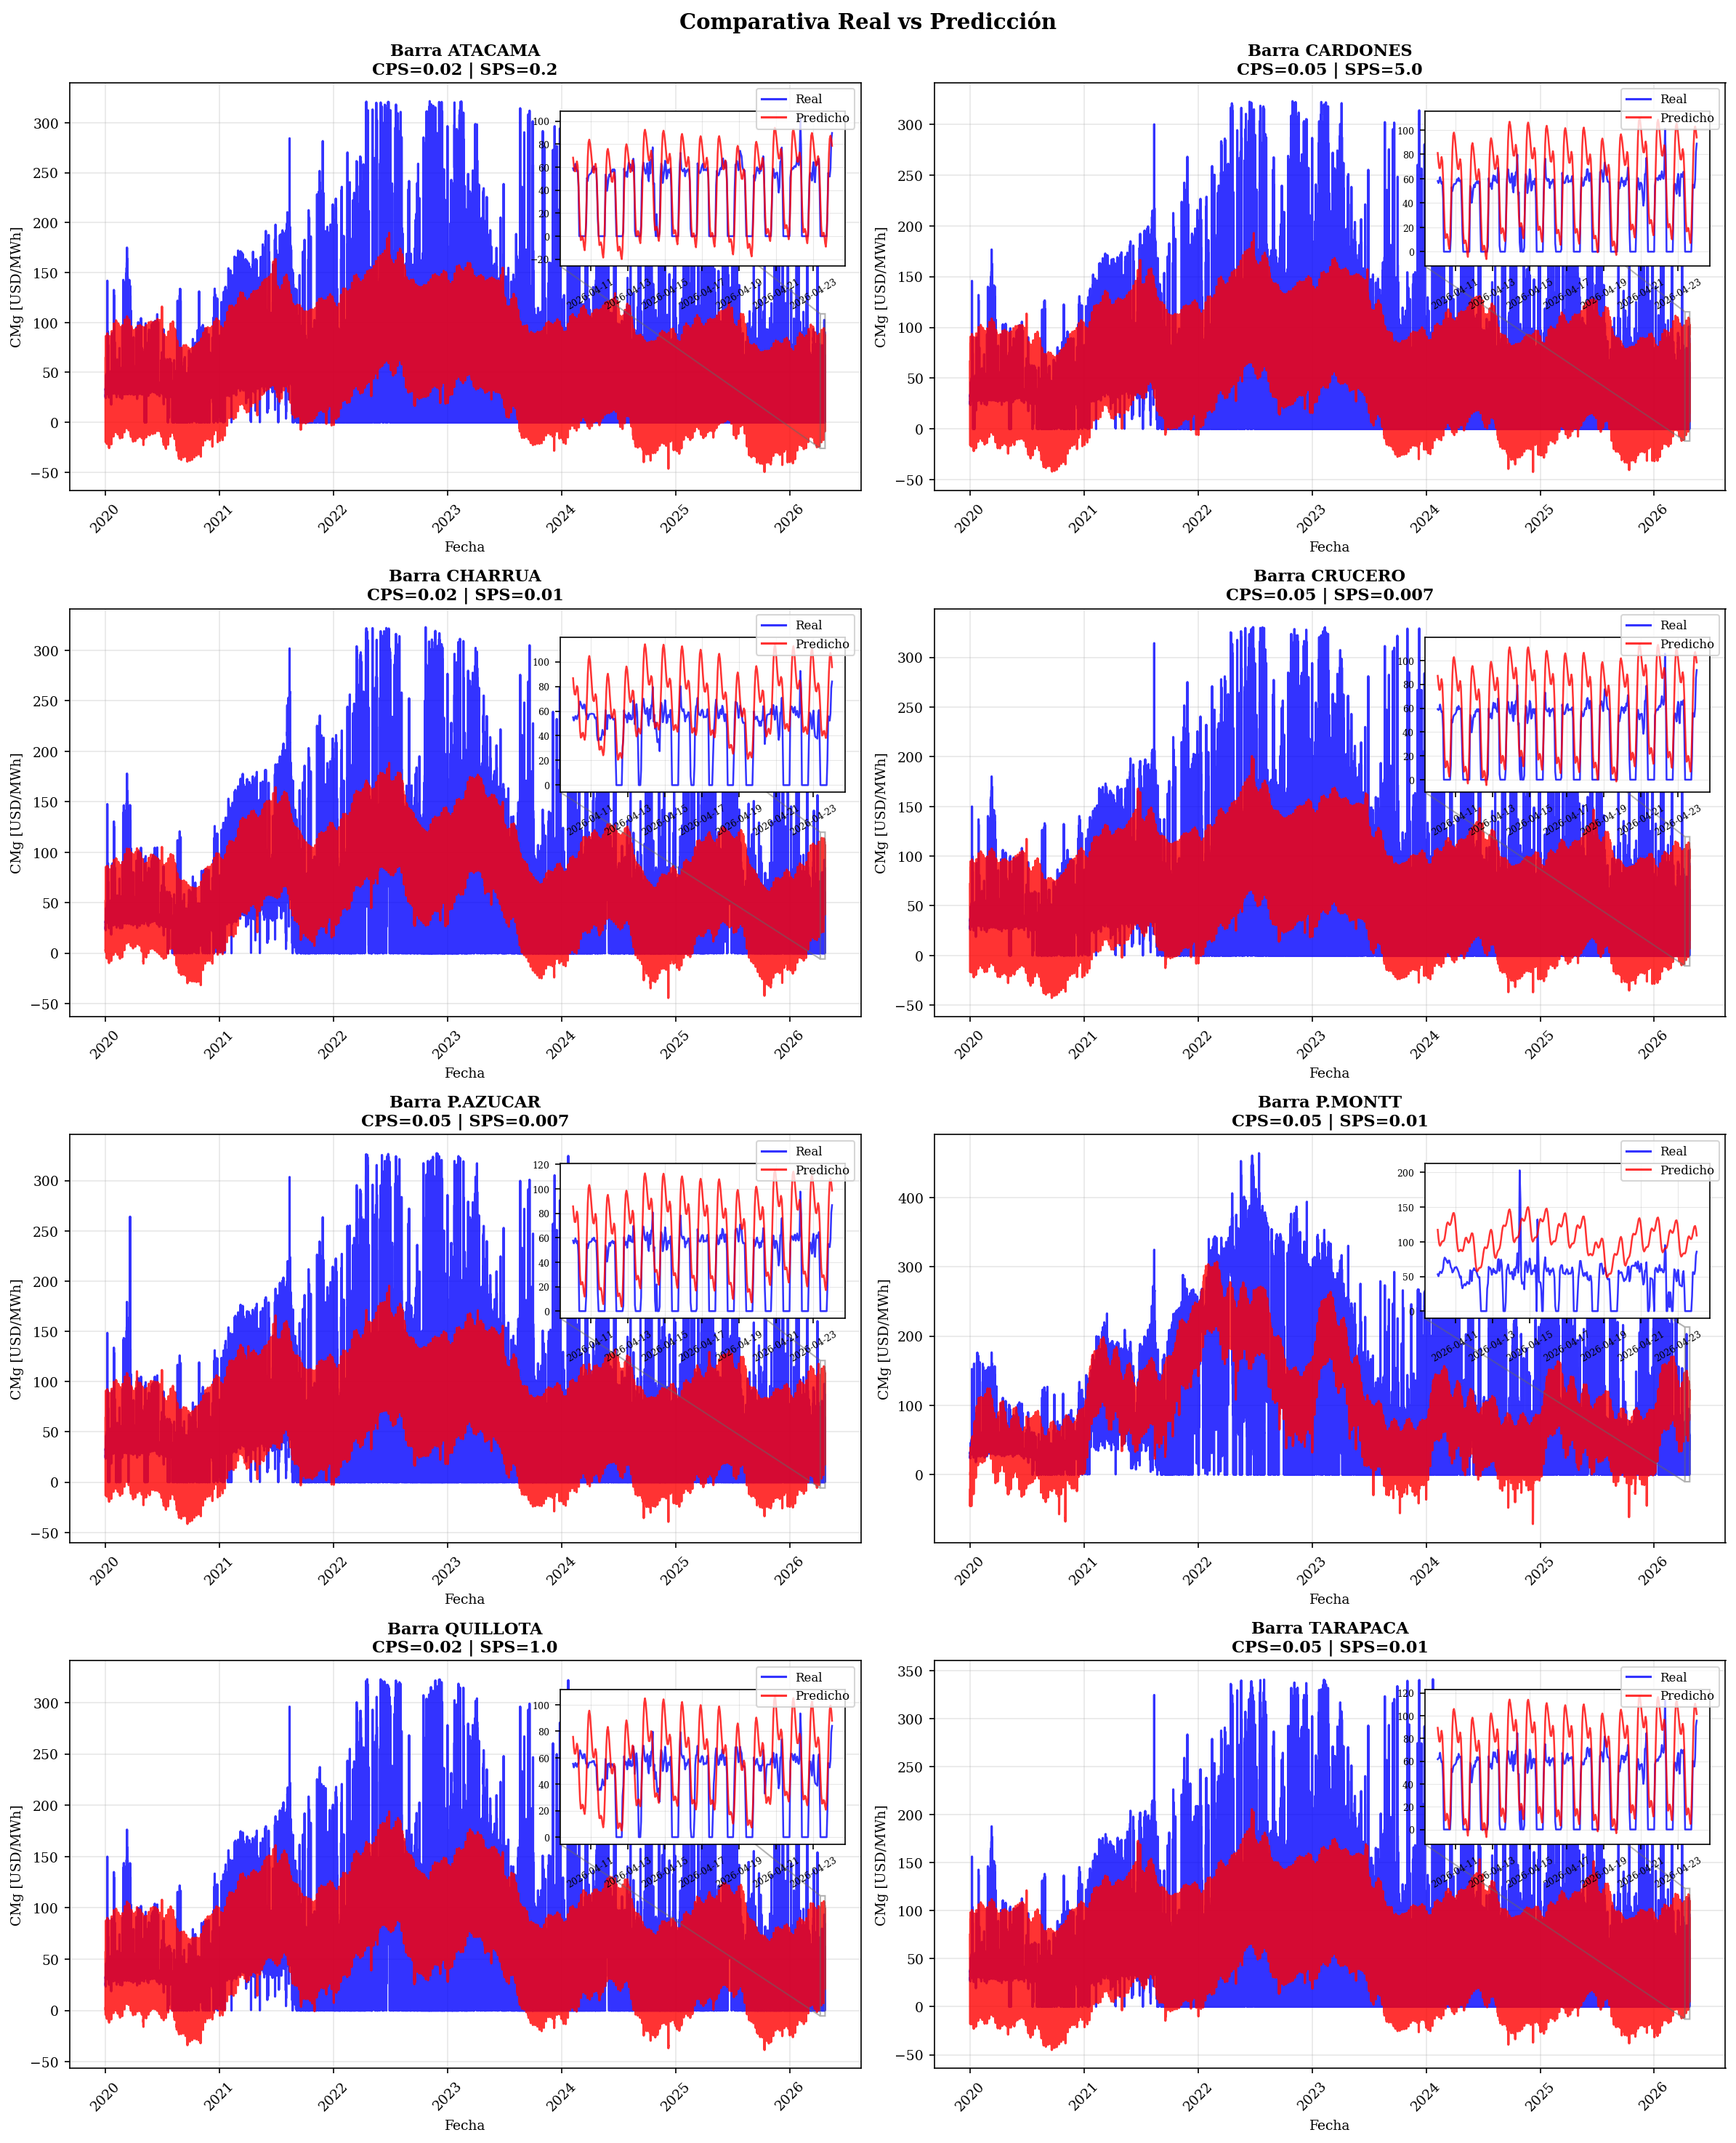
\includegraphics[width=0.95\textwidth]{imagenes/Posibles img/Comparativa Real vs Predicho.png}
    \caption{Comparativa entre valores reales (azul) y predicciones de Prophet (rojo) para las ocho barras del SEN, período 2020--2026.}
    \label{fig:prophet_comparativa}
\end{figure}

La figura ilustra visualmente el comportamiento característico de Prophet como modelo de descomposición: captura adecuadamente la envolvente de la serie, siguiendo la tendencia de largo plazo y los ciclos estacionales, pero suaviza los spikes de alta magnitud que corresponden a eventos extremos del mercado. Este comportamiento es esperable dado que Prophet modela la estructura sistemática de la serie y no está diseñado para capturar fluctuaciones no lineales de corto plazo, rol que corresponde al TFT en la arquitectura híbrida propuesta. Puerto Montt exhibe el mayor desajuste visual, con la predicción incapaz de seguir la alta variabilidad de la serie real durante el período 2022--2023.

La Tabla \ref{tab:prophet_resultados} presenta los resultados numéricos de evaluación de Prophet en los conjuntos de entrenamiento, validación y prueba para las ocho barras.

\begin{table}[htbp]
    \centering
    \small
    \begin{tabular}{llrrrr}
        \toprule
        Barra & Conjunto & MAE & RMSE & MSE & R$^2$ \\
        \midrule
        \multirow{3}{*}{Atacama}
            & Train & 30.40 & 41.05 & 1684.75 &  0.5228 \\
            & Val   & 21.34 & 42.29 & 1788.58 &  0.4023 \\
            & Test  & 16.39 & 28.69 &  823.05 &  0.5264 \\
        \midrule
        \multirow{3}{*}{Cardones}
            & Train & 30.32 & 40.92 & 1674.47 &  0.5314 \\
            & Val   & 21.60 & 37.21 & 1384.42 &  0.4491 \\
            & Test  & 19.95 & 30.09 &  905.28 &  0.4710 \\
        \midrule
        \multirow{3}{*}{Charrúa}
            & Train & 31.58 & 43.61 & 1901.89 &  0.4688 \\
            & Val   & 24.34 & 37.59 & 1412.72 &  0.3225 \\
            & Test  & 24.51 & 37.02 & 1370.68 &  0.3013 \\
        \midrule
        \multirow{3}{*}{Crucero}
            & Train & 30.46 & 41.23 & 1699.97 &  0.5502 \\
            & Val   & 22.83 & 42.13 & 1774.64 &  0.4167 \\
            & Test  & 22.10 & 31.94 & 1019.93 &  0.4238 \\
        \midrule
        \multirow{3}{*}{Pan de Azúcar}
            & Train & 30.83 & 41.98 & 1762.61 &  0.5137 \\
            & Val   & 22.73 & 37.21 & 1384.72 &  0.4161 \\
            & Test  & 22.44 & 31.79 & 1010.37 &  0.4137 \\
        \midrule
        \multirow{3}{*}{Puerto Montt}
            & Train & 50.44 & 67.62 & 4572.02 &  0.5516 \\
            & Val   & 46.00 & 62.88 & 3953.91 &  0.2221 \\
            & Test  & 47.89 & 61.71 & 3808.69 & $-$0.0106 \\
        \midrule
        \multirow{3}{*}{Quillota}
            & Train & 31.24 & 42.88 & 1838.39 &  0.4827 \\
            & Val   & 23.87 & 37.64 & 1416.80 &  0.3401 \\
            & Test  & 23.22 & 36.82 & 1355.75 &  0.3297 \\
        \midrule
        \multirow{3}{*}{Tarapacá}
            & Train & 31.18 & 42.20 & 1780.62 &  0.5568 \\
            & Val   & 23.61 & 43.97 & 1933.03 &  0.4355 \\
            & Test  & 21.86 & 32.88 & 1080.87 &  0.4692 \\
        \bottomrule
    \end{tabular}
    \vspace{0.2cm}
    \caption{Resultados de evaluación de Prophet por barra y conjunto, con las predicciones truncadas en 0 USD/MWh y validación/prueba evaluadas contra la serie cruda. MAE y RMSE en USD/MWh, MSE en (USD/MWh)$^2$.}
    \label{tab:prophet_resultados}
\end{table}

Los resultados muestran un desempeño heterogéneo entre barras. Las barras del norte presentan los mejores indicadores, con R$^2$ en el conjunto de prueba entre 0.41 y 0.53, lo que refleja que Prophet captura adecuadamente la estructura estacional y la tendencia decreciente asociada a la incorporación solar. Quillota y Charrúa muestran un desempeño moderado con R$^2$ de 0.33 y 0.30 respectivamente en prueba, sugiriendo que sus dinámicas de corto plazo son más difíciles de capturar con un modelo de descomposición aditiva. El caso más notable es Puerto Montt, que presenta un R$^2$ negativo de $-0.011$ en el conjunto de prueba, indicando que Prophet es peor que un predictor constante igual a la media para esta barra en el período 2025--2026. Este resultado es consistente con la naturaleza de la generación hidroeléctrica del sur, cuya variabilidad está determinada por ciclos de precipitaciones de baja frecuencia que no siguen patrones estacionales regulares. Este resultado motiva directamente la incorporación del TFT como componente complementario en el ensamble.

Las predicciones de Prophet se truncan en 0 USD/MWh antes de calcular estas métricas, dado que el costo marginal no puede ser negativo (Sección 3.3.3) y Prophet, como modelo de descomposición aditiva sin restricción de dominio, predice valores negativos con frecuencia no despreciable: 29\,346 de las 442\,560 predicciones evaluadas (6.6\%, sumando entrenamiento, validación y prueba en las ocho barras) son negativas antes de truncar. El efecto sobre las métricas es sistemático y no trivial --el MAE de prueba se reduce entre 0.3 (Puerto Montt) y 3.5\,USD/MWh (Atacama), y el R$^2$ de prueba mejora en las ocho barras, con la mayor ganancia en Atacama (0.484 a 0.526)--, consistente con que una fracción relevante de esas predicciones negativas ocurre en las horas de precio real cercano a 0 USD/MWh, donde el error absoluto de una predicción negativa es, por construcción, mayor que el de una predicción truncada en 0. Este truncamiento se aplica únicamente a las métricas de Prophet reportadas en esta sección; no se propaga al residuo que consume $\text{TFT}_\text{LN}$ en la rama P+C, dado que corregir ese residuo exige reentrenar el modelo de residuos sobre el nuevo objetivo, fuera del alcance de esta corrección puntual.

Se observa además una degradación consistente del R$^2$ entre entrenamiento y prueba en todas las barras, lo que es esperable dado el cambio estructural en el mercado eléctrico chileno durante el período de prueba 2025--2026, caracterizado por una mayor penetración renovable y episodios de curtailment más frecuentes que los observados durante el entrenamiento.

\section{Temporal Fusion Transformer con LayerNorm}
 
\subsection{Desempeño por barra}
 
Las Tablas \ref{tab:tft_precios_resultados} y \ref{tab:tft_residuos_resultados} presentan los resultados de evaluación del $\text{TFT}_\text{LN}$ para todas las barras, separados por modelo de precios y de residuos respectivamente.
 
\begin{table}[htbp]
    \centering
    \small
    \begin{tabular}{llrrr}
        \toprule
        Barra & Conjunto & MAE & RMSE & R$^2$ \\
        \midrule
        \multirow{3}{*}{Atacama}
            & Train & 7.81 & 16.30 & 0.925 \\
            & Val   & 8.95 & 29.32 & 0.713 \\
            & Test  & 6.95 & 16.93 & 0.835 \\
        \midrule
        \multirow{3}{*}{Cardones}
            & Train & 7.70 & 16.24 & 0.926 \\
            & Val   & 8.15 & 24.08 & 0.769 \\
            & Test  & 7.02 & 16.11 & 0.848 \\
        \midrule
        \multirow{3}{*}{Charrúa}
            & Train & 8.12 & 16.77 & 0.922 \\
            & Val   & 8.83 & 23.61 & 0.733 \\
            & Test  & 8.52 & 16.12 & 0.868 \\
        \midrule
        \multirow{3}{*}{Crucero}
            & Train & 7.80 & 16.34 & 0.930 \\
            & Val   & 8.80 & 28.50 & 0.733 \\
            & Test  & 7.06 & 16.92 & 0.838 \\
        \midrule
        \multirow{3}{*}{Pan de Azúcar}
            & Train & 7.57 & 15.80 & 0.931 \\
            & Val   & 8.36 & 23.26 & 0.772 \\
            & Test  & 7.17 & 15.33 & 0.864 \\
        \midrule
        \multirow{3}{*}{Puerto Montt}
            & Train & 13.01 & 29.70 & 0.914 \\
            & Val   & 15.80 & 33.19 & 0.783 \\
            & Test  & 13.94 & 25.98 & 0.821 \\
        \midrule
        \multirow{3}{*}{Quillota}
            & Train & 8.10 & 16.66 & 0.922 \\
            & Val   & 8.99 & 23.82 & 0.736 \\
            & Test  & 8.70 & 16.54 & 0.865 \\
        \midrule
        \multirow{3}{*}{Tarapacá}
            & Train & 7.91 & 16.63 & 0.931 \\
            & Val   & 9.17 & 31.08 & 0.718 \\
            & Test  & 7.14 & 17.90 & 0.843 \\
        \bottomrule
    \end{tabular}
    \vspace{0.2cm}
    \caption{Resultados de evaluación del $\text{TFT}_\text{LN}$, modelo de precios (rama P+C), por barra y conjunto, evaluado contra la serie cruda (Val y Test; Train se limpia igual que antes, Sección \ref{sec:baselines}). MAE y RMSE en USD/MWh.}
    \label{tab:tft_precios_resultados}
\end{table}
 
\begin{table}[htbp]
    \centering
    \small
    \begin{tabular}{llrrr}
        \toprule
        Barra & Conjunto & MAE & RMSE & R$^2$ \\
        \midrule
        \multirow{3}{*}{Atacama}
            & Train & 7.61 & 15.65 & 0.857 \\
            & Val   & 8.98 & 28.50 & 0.544 \\
            & Test  & 7.50 & 16.97 & 0.672 \\
        \midrule
        \multirow{3}{*}{Cardones}
            & Train & 7.55 & 15.48 & 0.860 \\
            & Val   & 8.10 & 23.66 & 0.600 \\
            & Test  & 6.80 & 15.39 & 0.736 \\
        \midrule
        \multirow{3}{*}{Charrúa}
            & Train & 8.21 & 16.66 & 0.855 \\
            & Val   & 8.81 & 23.29 & 0.618 \\
            & Test  & 8.46 & 15.62 & 0.823 \\
        \midrule
        \multirow{3}{*}{Crucero}
            & Train & 7.75 & 15.83 & 0.856 \\
            & Val   & 8.99 & 28.62 & 0.540 \\
            & Test  & 7.05 & 16.82 & 0.686 \\
        \midrule
        \multirow{3}{*}{Pan de Azúcar}
            & Train & 8.04 & 16.31 & 0.851 \\
            & Val   & 8.55 & 23.20 & 0.612 \\
            & Test  & 7.22 & 14.92 & 0.757 \\
        \midrule
        \multirow{3}{*}{Puerto Montt}
            & Train & 12.73 & 29.52 & 0.811 \\
            & Val   & 16.08 & 33.28 & 0.718 \\
            & Test  & 14.31 & 26.07 & 0.822 \\
        \midrule
        \multirow{3}{*}{Quillota}
            & Train & 8.28 & 16.60 & 0.851 \\
            & Val   & 9.38 & 23.85 & 0.600 \\
            & Test  & 8.95 & 16.56 & 0.795 \\
        \midrule
        \multirow{3}{*}{Tarapacá}
            & Train & 7.99 & 16.35 & 0.853 \\
            & Val   & 9.31 & 30.39 & 0.526 \\
            & Test  & 7.25 & 17.68 & 0.690 \\
        \bottomrule
    \end{tabular}
    \vspace{0.2cm}
    \caption{Resultados de evaluación del $\text{TFT}_\text{LN}$, modelo de residuos (rama P+C), por barra y conjunto, evaluado contra el residuo reconstruido a partir de la serie cruda (Val y Test; Train se limpia igual que antes, Sección \ref{sec:baselines}). MAE y RMSE en USD/MWh.}
    \label{tab:tft_residuos_resultados}
\end{table}
 
Los resultados muestran una mejora sustancial respecto a Prophet en todas las barras y métricas, evaluados contra la serie cruda (Sección \ref{sec:baselines}). En el $\text{TFT}_\text{LN}$ de precios, el R$^2$ en test oscila entre $0.821$ (Puerto Montt) y $0.868$ (Charrúa), frente a valores de Prophet que iban de $-0.016$ a $0.519$. Para Atacama, el R$^2$ sube de $0.519$ con Prophet a $0.835$ con el modelo de precios. El salto es especialmente pronunciado en Charrúa, de $0.302$ con Prophet a $0.868$ con el $\text{TFT}_\text{LN}$ de precios, y en Puerto Montt, de $-0.016$ a $0.821$, las dos barras con peor desempeño de Prophet, lo que confirma que el TFT es capaz de capturar las dinámicas no lineales de corto plazo que la descomposición aditiva de Prophet no puede representar.

Siete de las ocho barras presentan un MAE en test inferior a 9\,USD/MWh en el modelo de precios, con valores entre 6.95\,USD/MWh (Atacama) y 8.70\,USD/MWh (Quillota). Puerto Montt es la excepción, con un MAE de 13.94\,USD/MWh en test, consistente con la mayor variabilidad estructural de la generación hidroeléctrica del sur que ya se observaba en los resultados de Prophet. Aun así, el R$^2$ de $0.821$ en prueba indica que el $\text{TFT}_\text{LN}$ logra capturar una fracción importante de la dinámica de esta barra, a diferencia de Prophet que resultaba peor que un predictor constante.

El modelo de residuos presenta un R$^2$ en test entre $0.672$ (Atacama) y $0.823$ (Charrúa), sistemáticamente inferior al del modelo de precios en todas las barras, lo que es esperable: al operar sobre los residuos de Prophet, $\text{TFT}_\text{LN}$ modela una señal de menor amplitud y mayor irregularidad relativa.\footnote{Un bug en \texttt{Modulos/Stacking\_Optimization\_TFT.py} hacía que el cálculo de esta métrica comparara la predicción en escala de residuo contra el precio real en vez del residuo real, produciendo cifras no interpretables (MAE $\approx$ 44, R$^2$ negativo) al recalcularla sobre la corrida vigente del pipeline. El bug no afectaba a las estrategias de Stacking, que sí reconstruyen el precio completo (Tabla \ref{tab:mejores_estrategias}) y usan el residuo real correctamente en el resto del código; fue corregido, y las cifras de esta tabla se recalcularon directamente a partir de las predicciones y los residuos reales ya almacenados por el pipeline, sin necesidad de reentrenar ni re-ejecutar la optimización de Stacking completa. Posteriormente, para corregir el recorte de outliers (Sección \ref{sec:baselines}), el residuo real de val/test se reconstruyó restando la predicción de Prophet a la serie de precios cruda, en vez de usar el residuo ya recortado que almacenaba el pipeline.} Las métricas de error absoluto reportadas son comparables entre ambos modelos, con diferencias en MAE menores a 1.5\,USD/MWh en la mayoría de las barras, lo que indica que ambas instancias del Transformer aportan información complementaria al ensamble y justifica su inclusión conjunta en el Stacking Optimization.

\subsection{Sol+Clima (S+C)}

La rama S+C, descrita en la Sección 3.4.1, reemplaza las componentes de Prophet por variables de posición solar y prescinde tanto de Prophet como del modelo de residuos: se entrena una única instancia del TFT sobre la serie de precios. La Tabla \ref{tab:tft_sc_ln_resultados} presenta sus resultados para $\text{TFT}_\text{LN}$.

\begin{table}[htbp]
    \centering
    \small
    \begin{tabular}{llrrrrr}
        \toprule
        Barra & Conjunto & MAE & RMSE & R$^2$ & MASE & Skill \\
        \midrule
        \multirow{3}{*}{Atacama}
            & Train & 7.63 & 16.02 & 0.927 & & \\
            & Val   & 8.32 & 27.65 & 0.745 & & \\
            & Test  & 6.70 & 16.52 & 0.843 & 0.648 & 0.352 \\
        \midrule
        \multirow{3}{*}{Cardones}
            & Train & 7.92 & 16.48 & 0.924 & & \\
            & Val   & 7.73 & 23.17 & 0.786 & & \\
            & Test  & 6.63 & 15.61 & 0.858 & 0.641 & 0.359 \\
        \midrule
        \multirow{3}{*}{Charrúa}
            & Train & 8.04 & 16.56 & 0.923 & & \\
            & Val   & 8.43 & 23.17 & 0.743 & & \\
            & Test  & 7.98 & 15.32 & 0.880 & 0.776 & 0.224 \\
        \midrule
        \multirow{3}{*}{Crucero}
            & Train & 7.88 & 16.31 & 0.930 & & \\
            & Val   & 8.33 & 27.52 & 0.751 & & \\
            & Test  & 6.74 & 16.64 & 0.844 & 0.647 & 0.353 \\
        \midrule
        \multirow{3}{*}{Pan de Azúcar}
            & Train & 7.97 & 16.50 & 0.925 & & \\
            & Val   & 8.10 & 22.94 & 0.778 & & \\
            & Test  & 6.93 & 15.09 & 0.868 & 0.667 & 0.333 \\
        \midrule
        \multirow{3}{*}{Puerto Montt}
            & Train & 12.43 & 29.06 & 0.917 & & \\
            & Val   & 15.46 & 32.93 & 0.787 & & \\
            & Test  & 13.68 & 25.80 & 0.823 & 0.964 & 0.036 \\
        \midrule
        \multirow{3}{*}{Quillota}
            & Train & 7.89 & 16.35 & 0.925 & & \\
            & Val   & 8.63 & 23.48 & 0.743 & & \\
            & Test  & 8.26 & 15.90 & 0.875 & 0.794 & 0.206 \\
        \midrule
        \multirow{3}{*}{Tarapacá}
            & Train & 8.17 & 16.89 & 0.929 & & \\
            & Val   & 8.94 & 30.14 & 0.735 & & \\
            & Test  & 7.11 & 17.77 & 0.845 & 0.643 & 0.357 \\
        \bottomrule
    \end{tabular}
    \vspace{0.2cm}
    \caption{Resultados de evaluación del $\text{TFT}_\text{LN}$, rama S+C (única instancia, sin residuos), por barra y conjunto, evaluados contra la serie cruda sin recorte de outliers (Val y Test; Train se limpia igual que antes para estabilizar el entrenamiento, Sección \ref{sec:baselines}). MAE y RMSE en USD/MWh. MASE y Skill score respecto a la persistencia de un paso (Tabla \ref{tab:baselines_naive}), reportados solo para Test.}
    \label{tab:tft_sc_ln_resultados}
\end{table}

Comparando directamente contra el $\text{TFT}_\text{LN}$ de precios de la rama P+C (Tabla \ref{tab:tft_precios_resultados}), S+C obtiene menor MAE en test en las ocho barras, con mejoras de entre 0.4\% (Tarapacá, un margen mínimo) y 6.3\% (Charrúa). Esto ocurre pese a que S+C es, por diseño, un modelo más simple: no requiere ajustar Prophet ni entrenar una segunda instancia del TFT sobre residuos. La Sección \ref{sec:pc_vs_sc} retoma esta comparación de forma sistemática, incluyendo las estrategias de Stacking de P+C, que sí logran superar a S+C en algunos casos puntuales.

\section{Stacking Optimization}

\subsection{Selección del mejor método de optimización}

Se compararon ocho métodos numéricos (\textit{Grid Search} con 21, 41 y 101 puntos, \textit{Differential Evolution}, L-BFGS-B, Nelder-Mead, \textit{Random Search} con 1\,000 muestras, y SLSQP) para el mismo problema de un grado de libertad ($w_1$, con $w_2=1-w_1$) sobre la función objetivo MAE, más Ridge como comparación aparte: Ridge no optimiza ese mismo objetivo, sino que resuelve en forma cerrada un problema distinto (mínimos cuadrados con penalización $\ell_2$), por lo que se incluyó para verificar que un estimador de uso común no se aleja del resultado de los ocho anteriores, no como un noveno optimizador del mismo problema. Al ser MAE convexa y unimodal en una variable, era esperable que los ocho métodos numéricos convergieran al mismo mínimo, y en efecto lo hacen: las diferencias de MAE entre métodos son inferiores al 0.1\% en las 24 combinaciones de barra y estrategia evaluadas, y Ridge no se aparta de ese mismo óptimo de forma apreciable pese a resolver un problema distinto. La única diferencia práctica es el tiempo de cómputo (\textit{Random Search} el más lento, 0.6--1.2\,s; SLSQP y Ridge los más rápidos, bajo 0.05\,s en la mayoría de las barras), irrelevante a esta escala. Dado que la elección de método no afecta la calidad del ensamble, los resultados reportados en el resto de esta sección emplean indistintamente el método con menor MAE de cada barra y estrategia.

\subsection{Selección de la mejor estrategia}

La Tabla \ref{tab:mejores_estrategias} presenta la mejor estrategia por barra según el MAE en \textbf{validación} (Sección \ref{sec:baselines}), incluyendo los pesos aprendidos y la mejora porcentual en el conjunto de prueba, evaluado contra la serie cruda, respecto a Prophet solo y al $\text{TFT}_\text{LN}$ de precios solo.

\begin{table}[htbp]
    \centering
    \small
    \begin{tabular}{llllrr}
        \toprule
        Barra & Mejor estrategia & Pesos & MAE & $\Delta$Prophet & $\Delta$TFT \\
        \midrule
        Atacama        & (P$+$R) $+$ TFT precios  & $w_1{=}0.623,\,w_2{=}0.377$ & 7.10  & 64.27\% & $-2.17\%$ \\
        Cardones       & (P$+$R) $+$ TFT precios  & $w_1{=}0.598,\,w_2{=}0.402$ & 6.73  & 68.65\% & 4.14\% \\
        Charrúa        & (P$+$R) $+$ TFT precios  & $w_1{=}0.427,\,w_2{=}0.573$ & 8.32  & 67.19\% & 2.43\% \\
        Crucero        & (P$+$R) $+$ TFT precios  & $w_1{=}0.549,\,w_2{=}0.451$ & 6.86  & 70.27\% & 2.87\% \\
        Pan de Azúcar  & (P$+$R) $+$ TFT precios  & $w_1{=}0.206,\,w_2{=}0.794$ & 7.05  & 69.49\% & 1.76\% \\
        Puerto Montt   & TFT precios solo         & ---                         & 13.94 & 71.05\% & 0.00\%   \\
        Quillota       & (P$+$R) $+$ TFT precios  & $w_1{=}0.402,\,w_2{=}0.598$ & 8.62  & 64.52\% & 1.00\% \\
        Tarapacá       & (P$+$R) $+$ TFT precios  & $w_1{=}0.427,\,w_2{=}0.573$ & 7.06  & 69.56\% & 1.17\% \\
        \bottomrule
    \end{tabular}
    \vspace{0.2cm}
    \caption{Mejor estrategia de ensamblaje con $\text{TFT}_\text{LN}$ por barra, seleccionada por MAE en validación y evaluada contra la serie cruda. (P$+$R): Prophet$+$residuos; $w_1$ es el peso de (P$+$R), $w_2$ el del TFT de precios. MAE en USD/MWh. $\Delta$Prophet y $\Delta$TFT indican la mejora porcentual en MAE de prueba respecto a Prophet solo y al $\text{TFT}_\text{LN}$ de precios solo respectivamente; un valor negativo indica que la estrategia elegida en validación resulta, por azar, ligeramente peor en prueba que la alternativa más simple.}
    \label{tab:mejores_estrategias}
\end{table}

Los resultados revelan patrones similares a los de una selección por test, con una diferencia importante. Primero, el ensamble supera a Prophet en las ocho barras con mejoras de entre el 64.3\% (Atacama) y el 71.1\% (Puerto Montt) en MAE, confirmando que la combinación de modelos aporta valor significativo respecto a la descomposición temporal por sí sola. Segundo, en Puerto Montt la mejor estrategia es el $\text{TFT}_\text{LN}$ de precios solo; en las siete barras restantes gana (Prophet $+$ residuos) $+$ TFT precios, con mejoras de hasta 4.1\% (Cardones) respecto al TFT solo. Tercero, y a diferencia de una selección por test --que por construcción nunca puede rendir peor que la alternativa más simple--, en Atacama la estrategia elegida en validación resulta 2.2\% \emph{peor} que el TFT solo una vez evaluada en prueba: es el costo esperable de seleccionar sin mirar el conjunto de evaluación, y una ilustración directa de por qué la selección en test inflaba artificialmente estos números en la versión anterior de esta tabla.

Cabe destacar que la estrategia Prophet$+$residuos optimizada presenta un MAE significativamente mayor que las demás estrategias en todas las barras (14--36\,USD/MWh frente a 6--14\,USD/MWh), lo que sugiere que los residuos del TFT por sí solos, sin el anclaje del TFT de precios, no constituyen una señal suficientemente informativa para el ensamble. Esta observación refuerza el rol del $\text{TFT}_\text{LN}$ de precios como componente dominante del modelo híbrido.

\section{Temporal Fusion Transformer con Dynamic Tanh}

\subsection{Desempeño por barra}

Las Tablas \ref{tab:tft_dyt_precios_resultados} y \ref{tab:tft_dyt_residuos_resultados} presentan los resultados de evaluación del $\text{TFT}_\text{DyT}$ para todas las barras, separados por modelo de precios y de residuos respectivamente.

\begin{table}[htbp]
    \centering
    \small
    \begin{tabular}{llrrr}
        \toprule
        Barra & Conjunto & MAE & RMSE & R$^2$ \\
        \midrule
        \multirow{3}{*}{Atacama}
            & Train & 7.49 & 14.79 & 0.938 \\
            & Val   & 9.05 & 28.67 & 0.725 \\
            & Test  & 7.25 & 17.14 & 0.831 \\
        \midrule
        \multirow{3}{*}{Cardones}
            & Train & 7.49 & 14.62 & 0.940 \\
            & Val   & 8.25 & 23.99 & 0.771 \\
            & Test  & 7.11 & 16.31 & 0.845 \\
        \midrule
        \multirow{3}{*}{Charrúa}
            & Train & 7.91 & 15.09 & 0.936 \\
            & Val   & 9.14 & 23.72 & 0.730 \\
            & Test  & 8.73 & 15.97 & 0.870 \\
        \midrule
        \multirow{3}{*}{Crucero}
            & Train & 7.96 & 15.82 & 0.934 \\
            & Val   & 9.00 & 28.47 & 0.734 \\
            & Test  & 7.21 & 17.09 & 0.835 \\
        \midrule
        \multirow{3}{*}{Pan de Azúcar}
            & Train & 8.16 & 15.72 & 0.932 \\
            & Val   & 8.65 & 23.35 & 0.770 \\
            & Test  & 7.31 & 15.33 & 0.864 \\
        \midrule
        \multirow{3}{*}{Puerto Montt}
            & Train & 10.63 & 24.19 & 0.943 \\
            & Val   & 15.77 & 32.43 & 0.793 \\
            & Test  & 13.97 & 25.51 & 0.827 \\
        \midrule
        \multirow{3}{*}{Quillota}
            & Train & 7.54 & 14.42 & 0.942 \\
            & Val   & 9.29 & 24.11 & 0.729 \\
            & Test  & 9.02 & 16.79 & 0.861 \\
        \midrule
        \multirow{3}{*}{Tarapacá}
            & Train & 7.63 & 15.03 & 0.944 \\
            & Val   & 9.52 & 31.20 & 0.716 \\
            & Test  & 7.50 & 18.39 & 0.834 \\
        \bottomrule
    \end{tabular}
    \vspace{0.2cm}
    \caption{Resultados de evaluación del $\text{TFT}_\text{DyT}$, modelo de precios (rama P+C), por barra y conjunto, evaluado contra la serie cruda (Val y Test; Train se limpia igual que antes, Sección \ref{sec:baselines}). MAE y RMSE en USD/MWh.}
    \label{tab:tft_dyt_precios_resultados}
\end{table}

\begin{table}[htbp]
    \centering
    \small
    \begin{tabular}{llrrr}
        \toprule
        Barra & Conjunto & MAE & RMSE & R$^2$ \\
        \midrule
        \multirow{3}{*}{Atacama}
            & Train & 7.55 & 14.46 & 0.878 \\
            & Val   & 10.64 & 29.49 & 0.512 \\
            & Test  & 8.98 & 18.27 & 0.619 \\
        \midrule
        \multirow{3}{*}{Cardones}
            & Train & 7.38 & 14.07 & 0.884 \\
            & Val   & 8.53 & 24.00 & 0.589 \\
            & Test  & 7.64 & 16.47 & 0.698 \\
        \midrule
        \multirow{3}{*}{Charrúa}
            & Train & 8.10 & 15.25 & 0.879 \\
            & Val   & 9.55 & 24.12 & 0.591 \\
            & Test  & 8.86 & 16.14 & 0.810 \\
        \midrule
        \multirow{3}{*}{Crucero}
            & Train & 7.50 & 14.41 & 0.881 \\
            & Val   & 9.47 & 28.74 & 0.536 \\
            & Test  & 7.67 & 17.59 & 0.657 \\
        \midrule
        \multirow{3}{*}{Pan de Azúcar}
            & Train & 7.62 & 14.46 & 0.883 \\
            & Val   & 8.88 & 23.88 & 0.589 \\
            & Test  & 7.35 & 15.54 & 0.736 \\
        \midrule
        \multirow{3}{*}{Puerto Montt}
            & Train & 10.86 & 23.99 & 0.875 \\
            & Val   & 16.21 & 33.03 & 0.723 \\
            & Test  & 14.34 & 25.73 & 0.827 \\
        \midrule
        \multirow{3}{*}{Quillota}
            & Train & 7.87 & 14.61 & 0.885 \\
            & Val   & 9.58 & 24.01 & 0.594 \\
            & Test  & 9.47 & 16.65 & 0.793 \\
        \midrule
        \multirow{3}{*}{Tarapacá}
            & Train & 7.77 & 14.66 & 0.882 \\
            & Val   & 10.28 & 31.63 & 0.486 \\
            & Test  & 8.63 & 18.75 & 0.652 \\
        \bottomrule
    \end{tabular}
    \vspace{0.2cm}
    \caption{Resultados de evaluación del $\text{TFT}_\text{DyT}$, modelo de residuos (rama P+C), por barra y conjunto, evaluado contra el residuo reconstruido a partir de la serie cruda (Val y Test; Train se limpia igual que antes, Sección \ref{sec:baselines}). MAE y RMSE en USD/MWh.}
    \label{tab:tft_dyt_residuos_resultados}
\end{table}

Los resultados del $\text{TFT}_\text{DyT}$ son cualitativamente equivalentes a los del $\text{TFT}_\text{LN}$ en todas las barras y métricas. En el modelo de precios, el R$^2$ en test oscila entre $0.827$ (Puerto Montt) y $0.870$ (Charrúa), rango comparable al de $0.821$--$0.868$ obtenido por $\text{TFT}_\text{LN}$. Siete de las ocho barras presentan un MAE en test inferior a $9$\,USD/MWh en el modelo de precios, con valores entre $7.11$\,USD/MWh (Cardones) y $8.73$\,USD/MWh (Charrúa). Puerto Montt sigue siendo la excepción con un MAE de $13.97$\,USD/MWh en test, consistente con la mayor variabilidad estructural de la generación hidroeléctrica del sur.

El modelo de residuos presenta, al igual que con $\text{TFT}_\text{LN}$, un R$^2$ sistemáticamente inferior al de precios en todas las barras, entre $0.619$ (Atacama) y $0.827$ (Puerto Montt) en test.\footnote{Al igual que con $\text{TFT}_\text{LN}$ (nota de la Sección 4.2), las cifras de la Tabla \ref{tab:tft_dyt_residuos_resultados} fueron recalculadas tras corregir el mismo bug de escala en \texttt{Modulos/Stacking\_Optimization\_TFT.py}, y posteriormente tras corregir el recorte de outliers reconstruyendo el residuo real a partir de la serie de precios cruda.} Las métricas de error absoluto reportadas son comparables entre el modelo de precios y el de residuos, con diferencias en MAE menores a $1.8$\,USD/MWh en la mayoría de las barras, lo que confirma que ambas instancias del TFT aportan información complementaria al ensamble independientemente del mecanismo de normalización utilizado.

No se observa un patrón sistemático respecto a qué modelo, precios o residuos, se desempeña mejor con $\text{TFT}_\text{DyT}$ en comparación con $\text{TFT}_\text{LN}$. En algunas barras DyT supera a LN en el modelo de precios pero no en el de residuos, y en otras ocurre lo contrario. Esta ausencia de patrón es consistente con la hipótesis de diversidad estructural planteada en la Sección 2.4.5: las diferencias entre ambas arquitecturas no reflejan una ventaja predictiva media sistemática sino patrones de error cualitativamente distintos ante eventos extremos, que es lo que el Stacking Optimization puede explotar para mejorar la predicción conjunta.

\subsection{Sol+Clima (S+C) con \texorpdfstring{$\text{TFT}_\text{DyT}$}{TFT DyT}}

La Tabla \ref{tab:tft_sc_dyt_resultados} presenta los resultados de la rama S+C para $\text{TFT}_\text{DyT}$, análoga a la Tabla \ref{tab:tft_sc_ln_resultados} de la Sección 4.2.2 para $\text{TFT}_\text{LN}$.

\begin{table}[htbp]
    \centering
    \small
    \begin{tabular}{llrrr}
        \toprule
        Barra & Conjunto & MAE & RMSE & R$^2$ \\
        \midrule
        \multirow{3}{*}{Atacama}
            & Train & 8.12 & 16.28 & 0.925 \\
            & Val   & 7.07 & 14.91 & 0.899 \\
            & Test  & 6.36 & 12.95 & 0.896 \\
        \midrule
        \multirow{3}{*}{Cardones}
            & Train & 7.73 & 15.47 & 0.933 \\
            & Val   & 7.11 & 14.98 & 0.890 \\
            & Test  & 6.55 & 13.47 & 0.888 \\
        \midrule
        \multirow{3}{*}{Charrúa}
            & Train & 7.88 & 15.50 & 0.933 \\
            & Val   & 8.04 & 15.60 & 0.857 \\
            & Test  & 8.06 & 14.91 & 0.880 \\
        \midrule
        \multirow{3}{*}{Crucero}
            & Train & 8.10 & 16.25 & 0.930 \\
            & Val   & 6.99 & 15.04 & 0.900 \\
            & Test  & 6.57 & 13.32 & 0.892 \\
        \midrule
        \multirow{3}{*}{Pan de Azúcar}
            & Train & 7.54 & 15.08 & 0.937 \\
            & Val   & 7.46 & 15.30 & 0.881 \\
            & Test  & 6.70 & 13.83 & 0.885 \\
        \midrule
        \multirow{3}{*}{Puerto Montt}
            & Train & 10.66 & 24.13 & 0.943 \\
            & Val   & 15.09 & 29.93 & 0.812 \\
            & Test  & 14.01 & 26.04 & 0.820 \\
        \midrule
        \multirow{3}{*}{Quillota}
            & Train & 7.61 & 14.82 & 0.938 \\
            & Val   & 8.11 & 15.60 & 0.862 \\
            & Test  & 8.29 & 15.05 & 0.880 \\
        \midrule
        \multirow{3}{*}{Tarapacá}
            & Train & 8.16 & 16.35 & 0.934 \\
            & Val   & 7.44 & 16.15 & 0.900 \\
            & Test  & 6.62 & 13.76 & 0.900 \\
        \bottomrule
    \end{tabular}
    \vspace{0.2cm}
    \caption{Resultados de evaluación del $\text{TFT}_\text{DyT}$, rama S+C, por barra y conjunto. MAE y RMSE en USD/MWh.}
    \label{tab:tft_sc_dyt_resultados}
\end{table}

El patrón es el mismo que con $\text{TFT}_\text{LN}$: S+C obtiene menor MAE en test que el $\text{TFT}_\text{DyT}$ de precios de P+C (Tabla \ref{tab:tft_dyt_precios_resultados}) en siete de las ocho barras, con mejoras de entre 4.7\% (Crucero) y 7.8\% (Atacama); la excepción es nuevamente Puerto Montt, aunque por un margen mínimo (0.3\%). La Sección \ref{sec:pc_vs_sc} sistematiza esta comparación considerando también las estrategias de Stacking.

\subsection{Stacking Optimization con $\text{TFT}_\text{DyT}$}

El procedimiento de Stacking Optimization descrito en la Sección 3.5 se repite íntegramente para $\text{TFT}_\text{DyT}$, evaluando las mismas seis estrategias de ensamblaje y los mismos ocho métodos numéricos de optimización de pesos más Ridge utilizados para $\text{TFT}_\text{LN}$. La Tabla \ref{tab:stacking_dyt_mejores} presenta la mejor estrategia por barra según el MAE en \textbf{validación}, evaluada en prueba contra la serie cruda.

\begin{table}[htbp]
    \centering
    \small
    \begin{tabular}{llllrr}
        \toprule
        Barra & Mejor estrategia & Pesos & MAE & $\Delta$Prophet & $\Delta$TFT \\
        \midrule
        Atacama        & TFT$_\text{DyT}$ precios solo  & ---                         & 7.25  & 63.51\% & 0.00\%    \\
        Cardones       & (P$+$R) $+$ TFT$_\text{DyT}$ P & $w_1{=}0.549,\,w_2{=}0.451$ & 7.18  & 66.54\% & $-1.01\%$ \\
        Charrúa        & (P$+$R) $+$ TFT$_\text{DyT}$ P & $w_1{=}0.427,\,w_2{=}0.573$ & 8.45  & 66.66\% & 3.21\% \\
        Crucero        & TFT$_\text{DyT}$ precios solo  & ---                         & 7.22  & 68.73\% & 0.00\%    \\
        Pan de Azúcar  & (P$+$R) $+$ TFT$_\text{DyT}$ P & $w_1{=}0.721,\,w_2{=}0.279$ & 7.08  & 69.35\% & 3.16\% \\
        Puerto Montt   & (P$+$R) $+$ TFT$_\text{DyT}$ P & $w_1{=}0.425,\,w_2{=}0.575$ & 13.71 & 71.53\% & 1.82\% \\
        Quillota       & (P$+$R) $+$ TFT$_\text{DyT}$ P & $w_1{=}0.353,\,w_2{=}0.647$ & 8.89  & 63.38\% & 1.43\% \\
        Tarapacá       & TFT$_\text{DyT}$ precios solo  & ---                         & 7.50  & 67.66\% & 0.00\%    \\
        \bottomrule
    \end{tabular}
    \vspace{0.2cm}
    \caption{Mejor estrategia de ensamblaje con $\text{TFT}_\text{DyT}$ por barra, seleccionada por MAE en validación y evaluada contra la serie cruda. P$+$R: Prophet $+$ Residuos; TFT$_\text{DyT}$ P: $\text{TFT}_\text{DyT}$ precios. $w_1$ es el peso de (P$+$R), $w_2$ el del TFT de precios. MAE en USD/MWh. $\Delta$Prophet y $\Delta$TFT indican la mejora porcentual en prueba respecto a Prophet solo y al $\text{TFT}_\text{DyT}$ de precios solo respectivamente; un valor negativo indica que la estrategia elegida en validación resulta, por azar, ligeramente peor en prueba.}
    \label{tab:stacking_dyt_mejores}
\end{table}

Los resultados revelan patrones similares a los de $\text{TFT}_\text{LN}$. Primero, la estrategia (Prophet $+$ residuos) $+$ TFT$_\text{DyT}$ precios domina en 5 de las 8 barras (Cardones, Charrúa, Pan de Azúcar, Puerto Montt y Quillota), mientras que en las 3 restantes (Atacama, Crucero y Tarapacá) el TFT solo es suficiente. Este reparto es parecido al observado en $\text{TFT}_\text{LN}$ (Tabla \ref{tab:mejores_estrategias}), donde el TFT solo gana únicamente en Puerto Montt: en ambas arquitecturas, la mayoría de las barras se beneficia de incorporar los residuos de Prophet.

Segundo, la mejora respecto a Prophet es consistente y grande en todas las barras, entre $63.38\%$ (Quillota) y $71.53\%$ (Puerto Montt) en MAE, magnitud prácticamente idéntica a la obtenida con $\text{TFT}_\text{LN}$ ($64.27\%$--$71.05\%$), confirmando que el ensamble aporta valor significativo independientemente de la arquitectura de normalización.

Tercero, en Cardones el ensamble elegido en validación resulta 1.0\% peor que el TFT solo en prueba, el mismo efecto de selección honesta observado en Atacama bajo $\text{TFT}_\text{LN}$: no es un error, es evidencia de que la selección ya no está sesgada por el conjunto de evaluación. En las barras donde el ensamble sí mejora sobre el TFT solo, la magnitud es comparable entre arquitecturas (1.4\%--3.2\% en DyT frente a 1.0\%--4.1\% en LN), sin que una arquitectura muestre sistemáticamente mayor beneficio de incorporar los residuos de Prophet. Esto se retoma en la Sección \ref{sec:ln_vs_dyt}, y refuerza que ambas arquitecturas aportan diversidad complementaria al ensamble sin que una domine uniformemente a la otra.

Respecto a los métodos de optimización, el patrón es idéntico al observado con $\text{TFT}_\text{LN}$: las diferencias en MAE entre métodos para una misma estrategia y barra son inferiores al 0.1\%, con \textit{Random Search} consistentemente como el método más lento (0.5--1.1\,s) y Ridge/SLSQP entre los más rápidos. Esto confirma que la elección del método de optimización no constituye un grado de libertad relevante para los resultados del Stacking, independientemente de la arquitectura del TFT utilizada como componente del ensamble.

\subsection{Comparativa $\text{TFT}_\text{LN}$ vs.\ $\text{TFT}_\text{DyT}$}
\label{sec:ln_vs_dyt}

Esta subsección compara ambas arquitecturas de normalización en tres niveles: el desempeño puntual del TFT de precios en ambas ramas (P+C y S+C), la significancia estadística de las diferencias mediante una prueba de Diebold-Mariano pareada por hora, y el desempeño tras el Stacking Optimization, que es la comparación relevante para la elección final de arquitectura.

\subsubsection{Desempeño puntual}

La Tabla \ref{tab:ln_vs_dyt_test} presenta el MAE del TFT de precios para ambas ramas y arquitecturas, evaluado contra la serie cruda.

\begin{table}[htbp]
    \centering
    \small
    \begin{tabular}{lrrrr}
        \toprule
        & \multicolumn{2}{c}{P+C} & \multicolumn{2}{c}{S+C} \\
        \cmidrule(lr){2-3} \cmidrule(lr){4-5}
        Barra & LN & DyT & LN & DyT \\
        \midrule
        Atacama       & 6.95  & 7.25  & 6.70  & 6.68  \\
        Cardones      & 7.02  & 7.11  & 6.63  & 6.78  \\
        Charrúa       & 8.52  & 8.73  & 7.98  & 8.28  \\
        Crucero       & 7.06  & 7.21  & 6.74  & 6.87  \\
        Pan de Azúcar & 7.17  & 7.31  & 6.93  & 6.83  \\
        Puerto Montt  & 13.94 & 13.97 & 13.68 & 14.01 \\
        Quillota      & 8.70  & 9.02  & 8.26  & 8.58  \\
        Tarapacá      & 7.14  & 7.50  & 7.11  & 6.95  \\
        \bottomrule
    \end{tabular}
    \vspace{0.2cm}
    \caption{MAE de test del TFT de precios por rama y arquitectura, evaluado contra la serie cruda. USD/MWh.}
    \label{tab:ln_vs_dyt_test}
\end{table}

Las diferencias absolutas de MAE entre LN y DyT son pequeñas en todos los casos (inferiores a 0.5\,USD/MWh en la mayoría de las combinaciones), lo que en una primera lectura sugeriría equivalencia entre arquitecturas, en línea con lo reportado por Zhu et al.\ (2025) para otros dominios. Sin embargo, esta lectura basada en el promedio agregado (MAE) puede ser engañosa cuando la distribución de errores es asimétrica, como se muestra a continuación.

\subsubsection{Prueba de Diebold-Mariano pareada por hora}
\label{sec:dm_ln_dyt}

Para determinar si las diferencias observadas son sistemáticas u obedecen al azar, se compara la exactitud predictiva de LN y DyT mediante el test de Diebold-Mariano (1995) sobre los errores absolutos horarios del conjunto de prueba (evaluados contra la serie cruda, Sección \ref{sec:baselines}), para las 16 combinaciones de barra y rama (P+C y S+C). A diferencia de Wilcoxon, usado en una versión anterior de este análisis, Diebold-Mariano estima la varianza de la diferencia de pérdidas mediante Newey-West (con truncamiento $\text{lag}=h+1=2$, ponderación de Bartlett), lo que la hace robusta a la autocorrelación serial de los errores horarios --algo que Wilcoxon, al asumir observaciones independientes, no maneja, y que en este caso produce $p$-valores no interpretables (del orden de $10^{-40}$ a $10^{-50}$ para diferencias de MAE de apenas 0.1--0.4\,USD/MWh)--. El signo del estadístico DM indica directamente la dirección del efecto: negativo favorece a LN. La Tabla \ref{tab:dm_ln_dyt} presenta los resultados.

\begin{table}[htbp]
    \centering
    \small
    \begin{tabular}{llrrrrl}
        \toprule
        Barra & Rama & MAE$_\text{LN}$ & MAE$_\text{DyT}$ & DM & $p$ (dos colas) & Signif.\ (5\%) \\
        \midrule
        Atacama       & S+C & 6.705  & 6.683  & 0.46  & $0.644$              & No \\
        Cardones      & S+C & 6.626  & 6.777  & -2.81 & $5.0\times10^{-3}$  & Sí \\
        Charrúa       & S+C & 7.980  & 8.275  & -5.51 & $3.6\times10^{-8}$  & Sí \\
        Crucero       & S+C & 6.742  & 6.873  & -2.77 & $5.6\times10^{-3}$  & Sí \\
        Pan de Azúcar & S+C & 6.925  & 6.829  & 1.59  & $0.111$              & No \\
        Puerto Montt  & S+C & 13.684 & 14.011 & -2.73 & $6.3\times10^{-3}$  & Sí \\
        Quillota      & S+C & 8.265  & 8.576  & -4.95 & $7.4\times10^{-7}$  & Sí \\
        Tarapacá      & S+C & 7.115  & 6.953  & 2.89  & $3.9\times10^{-3}$  & Sí \\
        Atacama       & P+C & 6.945  & 7.247  & -4.41 & $1.0\times10^{-5}$  & Sí \\
        Cardones      & P+C & 7.016  & 7.106  & -1.29 & $0.196$              & No \\
        Charrúa       & P+C & 8.524  & 8.731  & -2.93 & $3.4\times10^{-3}$  & Sí \\
        Crucero       & P+C & 7.062  & 7.215  & -2.52 & $1.2\times10^{-2}$  & Sí \\
        Pan de Azúcar & P+C & 7.174  & 7.311  & -2.15 & $3.1\times10^{-2}$  & Sí \\
        Puerto Montt  & P+C & 13.939 & 13.965 & -0.23 & $0.821$              & No \\
        Quillota      & P+C & 8.702  & 9.020  & -3.71 & $2.0\times10^{-4}$  & Sí \\
        Tarapacá      & P+C & 7.141  & 7.498  & -5.56 & $2.7\times10^{-8}$  & Sí \\
        \bottomrule
    \end{tabular}
    \vspace{0.2cm}
    \caption{Test de Diebold-Mariano (varianza Newey-West, $\text{lag}=h+1=2$) entre los errores absolutos horarios de $\text{TFT}_\text{LN}$ y $\text{TFT}_\text{DyT}$, pareados por hora del conjunto de prueba, evaluados contra la serie cruda.}
    \label{tab:dm_ln_dyt}
\end{table}

En 12 de las 16 combinaciones la diferencia es estadísticamente significativa ($p<0.05$), es decir, no es atribuible al azar. El signo del estadístico DM muestra que $\text{TFT}_\text{LN}$ es el ganador en 11 de esas 12 combinaciones significativas; $\text{TFT}_\text{DyT}$ solo gana de forma significativa en Tarapacá bajo S+C. La ventaja de LN es unánime en la rama P+C (6 de 6 combinaciones significativas), y algo más mixta en S+C (5 de 6). En las 4 combinaciones restantes (Atacama y Pan de Azúcar bajo S+C, Cardones y Puerto Montt bajo P+C) el MAE nominal favorece a uno u otro por un margen pequeño, pero la diferencia no alcanza significancia estadística una vez que se descuenta la autocorrelación serial del error horario: no hay evidencia suficiente para preferir una arquitectura sobre la otra en esos casos específicos.

Una hipótesis para esta ventaja sistemática de LN, aunque de magnitud pequeña, es la diferencia estructural entre ambos mecanismos de normalización descrita en la Sección 2.4.4: LayerNorm recalcula la escala de activación de forma local, para cada paso temporal, mientras que DyT aplica un único escalar $\alpha$ global aprendido durante el entrenamiento. En una serie con heterocedasticidad horaria pronunciada como el costo marginal, la misma que motiva a LW-ACP en la Sección 2.6.4, esa adaptación local podría dar a LN una ventaja consistente aunque pequeña en la mayoría de las horas. Esta hipótesis es consistente con que la ventaja de LN no alcanza significancia precisamente en Puerto Montt bajo P+C, una de las barras con dinámicas de precio menos regidas por el ciclo solar diario.

\subsubsection{Comparativa tras el Stacking Optimization}

La Tabla \ref{tab:comparativa_stacking} presenta la comparación al nivel relevante para el modelo híbrido final: el MAE de la mejor estrategia de Stacking de P+C obtenida para cada arquitectura (Tablas \ref{tab:mejores_estrategias} y \ref{tab:stacking_dyt_mejores}), seleccionada en validación y evaluada en prueba contra la serie cruda.

\begin{table}[htbp]
    \centering
    \small
    \begin{tabular}{lrrrr}
        \toprule
        Barra & MAE Stacking LN & MAE Stacking DyT & Diferencia & Ganador \\
        \midrule
        Atacama       & 7.10  & 7.25  & 0.15 & LN  \\
        Cardones      & 6.73  & 7.18  & 0.45 & LN  \\
        Charrúa       & 8.32  & 8.45  & 0.13 & LN  \\
        Crucero       & 6.86  & 7.22  & 0.36 & LN  \\
        Pan de Azúcar & 7.05  & 7.08  & 0.03 & LN  \\
        Puerto Montt  & 13.94 & 13.71 & 0.23 & DyT \\
        Quillota      & 8.62  & 8.89  & 0.27 & LN  \\
        Tarapacá      & 7.06  & 7.50  & 0.44 & LN  \\
        \bottomrule
    \end{tabular}
    \vspace{0.2cm}
    \caption{MAE en prueba de la mejor estrategia de Stacking Optimization de P+C para cada arquitectura, por barra, evaluado contra la serie cruda. MAE en USD/MWh.}
    \label{tab:comparativa_stacking}
\end{table}

A nivel del ensamble final, $\text{TFT}_\text{LN}$ resulta ganador en 7 de las 8 barras, con Puerto Montt como única excepción a favor de $\text{TFT}_\text{DyT}$. Esto es consistente con la ventaja sistemática de LN detectada por el test de Diebold-Mariano: al ganar de forma típica hora a hora en la mayoría de las barras, LN también tiende a ganar el MAE agregado una vez que sus predicciones se combinan con las de Prophet en el Stacking. Las diferencias absolutas siguen siendo modestas (0.03--0.45\,USD/MWh sobre un MAE típico de 6--9\,USD/MWh), pero ya no son atribuibles únicamente a la variabilidad de inicialización, dado lo mostrado en la Tabla \ref{tab:dm_ln_dyt}.

La conclusión metodológica de esta sección es, entonces, más matizada que la de trabajos que reportan equivalencia estricta entre LayerNorm y DyT: en el contexto del pronóstico de precios eléctricos, $\text{TFT}_\text{LN}$ presenta una ventaja sistemática, aunque de magnitud pequeña, sobre $\text{TFT}_\text{DyT}$, particularmente marcada en la rama P+C. Esto no invalida el uso de DyT, sus diferencias con LN siguen siendo pequeñas en términos absolutos, y ambas arquitecturas exhiben patrones de error suficientemente distintos como para que su combinación en un ensamble más amplio (Stacking entre $\text{TFT}_\text{LN}$ y $\text{TFT}_\text{DyT}$, no explorado en este trabajo) sea una dirección de trabajo futuro razonable, pero sí sugiere que, si se debe elegir una única arquitectura de normalización para este problema, LayerNorm es la opción mejor respaldada por la evidencia.

\subsubsection{Robustez a la semilla de inicialización}
\label{sec:seeds_ln_dyt}

La comparación anterior se realiza bajo una única semilla de inicialización por modelo. Para acotar cuánto de la diferencia observada entre LN y DyT es atribuible a la variabilidad de inicialización y no a una diferencia sistemática entre arquitecturas, se repite el entrenamiento de S+C con 5 semillas distintas para tres barras piloto, manteniendo el resto de la configuración de la Tabla \ref{tab:tft_config} sin cambios. La Tabla \ref{tab:5seeds} presenta la media y desviación estándar del MAE de prueba sobre las 5 réplicas.

\begin{table}[htbp]
    \centering
    \begin{tabular}{lrrl}
        \toprule
        Barra & MAE$_\text{LN}$ (media $\pm$ sd) & MAE$_\text{DyT}$ (media $\pm$ sd) & ¿Se solapan? \\
        \midrule
        Atacama      & 6.631 $\pm$ 0.146  & 6.842 $\pm$ 0.113  & Sí \\
        Charrúa      & 8.081 $\pm$ 0.098  & 8.208 $\pm$ 0.061  & Sí \\
        Puerto Montt & 13.959 $\pm$ 0.295 & 13.774 $\pm$ 0.144 & Sí \\
        \bottomrule
    \end{tabular}
    \vspace{0.2cm}
    \caption{MAE de prueba (S+C, USD/MWh) sobre 5 semillas de inicialización, media $\pm$ desviación estándar. ``¿Se solapan?'' indica si los intervalos media $\pm$ 1 desviación estándar de LN y DyT se traslapan.}
    \label{tab:5seeds}
\end{table}

En las tres barras, los intervalos media $\pm$ 1 desviación estándar de LN y DyT se solapan completamente: la diferencia entre arquitecturas observada bajo una única semilla (Tabla \ref{tab:ln_vs_dyt_test}) es del mismo orden de magnitud que la variabilidad propia de la inicialización aleatoria. Esto no contradice la ventaja sistemática de LN establecida mediante el test de Diebold-Mariano (Sección \ref{sec:dm_ln_dyt}): ese test compara errores pareados hora a hora dentro de una misma semilla, una fuente de evidencia distinta y no afectada por la varianza entre semillas. Pero sí matiza su magnitud práctica --pequeña en comparación con el ruido de inicialización--, un matiz relevante para cualquier lectura que busque generalizar esta comparación más allá del pipeline específico de este trabajo. El resto de los experimentos de este capítulo, incluyendo las extensiones de las Secciones \ref{sec:piloto_outliers} y \ref{sec:h24_dayahead}, se entrenan sin semilla fija, igual que el pipeline principal; el control de semilla implementado para este estudio (\texttt{pl.seed\_everything}) no se propagó a esos entrenamientos posteriores.

\subsection{P+C vs.\ S+C: comparación central}
\label{sec:pc_vs_sc}

Las secciones anteriores presentaron P+C (Prophet+Clima, con Stacking Optimization) y S+C (Sol+Clima, instancia única del TFT) por separado. Esta subsección los compara directamente, tomando para P+C la mejor estrategia de Stacking de cada barra --seleccionada por MAE en \textbf{validación}, no en prueba (Sección \ref{sec:baselines}), y evaluada contra la serie cruda-- y para S+C su única predicción, también contra la serie cruda (Tablas \ref{tab:tft_sc_ln_resultados} y \ref{tab:tft_sc_dyt_resultados}). La Tabla \ref{tab:pc_vs_sc} presenta el resultado para las 16 combinaciones de barra y arquitectura, junto con el test de Diebold-Mariano (Sección \ref{sec:dm_ln_dyt}) sobre los errores absolutos horarios pareados.

\begin{table}[htbp]
    \centering
    \small
    \begin{tabular}{llrrlrrl}
        \toprule
        Barra & Arq. & MAE P+C & MAE S+C & Ganador & DM & $p$-valor & Signif.\ (5\%) \\
        \midrule
        Atacama       & LN  & 7.10  & 6.71  & S+C & 6.61  & $3.9\times10^{-11}$ & Sí \\
        Atacama       & DyT & 7.25  & 6.68  & S+C & 8.45  & $0$                  & Sí \\
        Cardones      & LN  & 6.73  & 6.63  & S+C & 1.93  & $0.053$              & No \\
        Cardones      & DyT & 7.18  & 6.78  & S+C & 6.07  & $1.3\times10^{-9}$  & Sí \\
        Charrúa       & LN  & 8.32  & 7.98  & S+C & 5.85  & $5.0\times10^{-9}$  & Sí \\
        Charrúa       & DyT & 8.45  & 8.28  & S+C & 2.61  & $9.2\times10^{-3}$  & Sí \\
        Crucero       & LN  & 6.86  & 6.74  & S+C & 2.22  & $0.026$              & Sí \\
        Crucero       & DyT & 7.22  & 6.87  & S+C & 5.72  & $1.1\times10^{-8}$  & Sí \\
        Pan de Azúcar & LN  & 7.05  & 6.93  & S+C & 1.92  & $0.055$              & No \\
        Pan de Azúcar & DyT & 7.08  & 6.83  & S+C & 3.47  & $5.3\times10^{-4}$  & Sí \\
        Puerto Montt  & LN  & 13.94 & 13.68 & S+C & 3.43  & $6.0\times10^{-4}$  & Sí \\
        Puerto Montt  & DyT & 13.71 & 14.01 & P+C & -2.59 & $9.7\times10^{-3}$  & Sí \\
        Quillota      & LN  & 8.62  & 8.26  & S+C & 5.48  & $4.3\times10^{-8}$  & Sí \\
        Quillota      & DyT & 8.89  & 8.58  & S+C & 3.84  & $1.3\times10^{-4}$  & Sí \\
        Tarapacá      & LN  & 7.06  & 7.11  & P+C & -1.12 & $0.263$              & No \\
        Tarapacá      & DyT & 7.50  & 6.95  & S+C & 7.70  & $1.4\times10^{-14}$ & Sí \\
        \bottomrule
    \end{tabular}
    \vspace{0.2cm}
    \caption{Comparación P+C (mejor estrategia de Stacking, seleccionada en validación) vs.\ S+C, MAE de test en USD/MWh, para las 8 barras y ambas arquitecturas, evaluado contra la serie cruda, con test de Diebold-Mariano (varianza Newey-West) sobre los errores absolutos horarios pareados. El signo de DM favorece a S+C cuando es positivo.}
    \label{tab:pc_vs_sc}
\end{table}

\textbf{S+C gana en 14 de las 16 combinaciones} por MAE nominal, con mejoras de entre 1.5\% (Cardones LN) y 7.9\% (Atacama DyT) respecto al MAE de P+C. Las únicas dos excepciones nominales son Tarapacá con LN y Puerto Montt con DyT. El test de Diebold-Mariano confirma que esta ventaja no es atribuible al azar en la mayoría de los casos: la diferencia es estadísticamente significativa en 13 de las 16 combinaciones, y S+C gana en 12 de esas 13 (92\%); la única combinación significativa a favor de P+C es Puerto Montt bajo DyT. En las 3 combinaciones restantes (Cardones y Pan de Azúcar bajo LN, Tarapacá bajo LN) la diferencia nominal de MAE no alcanza significancia estadística, es decir, no hay evidencia suficiente para preferir una rama sobre la otra en esos casos específicos --incluyendo la única excepción nominal de S+C bajo LN (Tarapacá), que en rigor no es una victoria significativa de P+C, sino una ausencia de diferencia detectable--. Este resultado es notable porque S+C es, por diseño, la estrategia más simple: prescinde de Prophet, de su ajuste por barra, y del modelo de residuos y el Stacking Optimization que P+C requiere para alcanzar su mejor desempeño. La ventaja de S+C es consistente en ambas arquitecturas y en siete de las ocho barras, lo que sugiere que la posición solar, calculada de forma determinista y exacta mediante \texttt{pvlib}, captura el ciclo diario y anual del costo marginal de manera al menos tan efectiva como la descomposición estadística de Prophet, sin acumular su error de ajuste ni requerir el paso adicional de ensamblaje. Puerto Montt, la única barra donde P+C es significativamente ganador en alguna arquitectura, es consistente con su menor dependencia del ciclo solar y su mayor dependencia de la disponibilidad hidroeléctrica, ya documentada en la Sección 4.7.1.

Este hallazgo, que la estrategia más simple es también la más precisa en la gran mayoría de los casos, es el resultado central de este trabajo, y motiva que S+C sea adoptada como estrategia de referencia en el resto de este capítulo. Combinado con la ventaja sistemática, aunque pequeña, de $\text{TFT}_\text{LN}$ sobre $\text{TFT}_\text{DyT}$ establecida en la Sección \ref{sec:ln_vs_dyt}, la selección final de este trabajo es \textbf{S+C-LN}: un único modelo, sin Stacking Optimization ni ajuste por barra, adoptado de forma uniforme en Conformal Prediction (Sección 4.5). Las extensiones de la Sección 4.7 retoman la comparación entre ambas arquitecturas donde es relevante para sus propios objetivos (por ejemplo, la robustez de la conclusión sobre Puerto Montt o el estudio de granularidad), en vez de asumir S+C-LN de antemano.

\section{Conformal Prediction}

Antes de presentar los resultados numéricos de cada método, la Figura \ref{fig:cp_ejemplo_intervalo} ilustra cómo se ve en la práctica un intervalo de predicción: un día del conjunto de prueba en Atacama, con el intervalo de LW-ACP (la variante finalmente seleccionada, Sección \ref{sec:lwacp_resultados}) superpuesto al precio real y a la predicción puntual de S+C-LN. Es un día representativo del comportamiento típico del intervalo, no necesariamente del ancho medio reportado más adelante (Sección \ref{sec:lwacp_resultados}), que promedia sobre todas las horas y los 8.298 días-hora del conjunto de prueba, incluyendo las horas de mayor volatilidad; con solo 24 observaciones, no cubrir ninguna en este día particular es un resultado perfectamente consistente con el 95\% de cobertura nominal, no evidencia de una selección atípicamente favorable.

\begin{figure}[htbp]
    \centering
    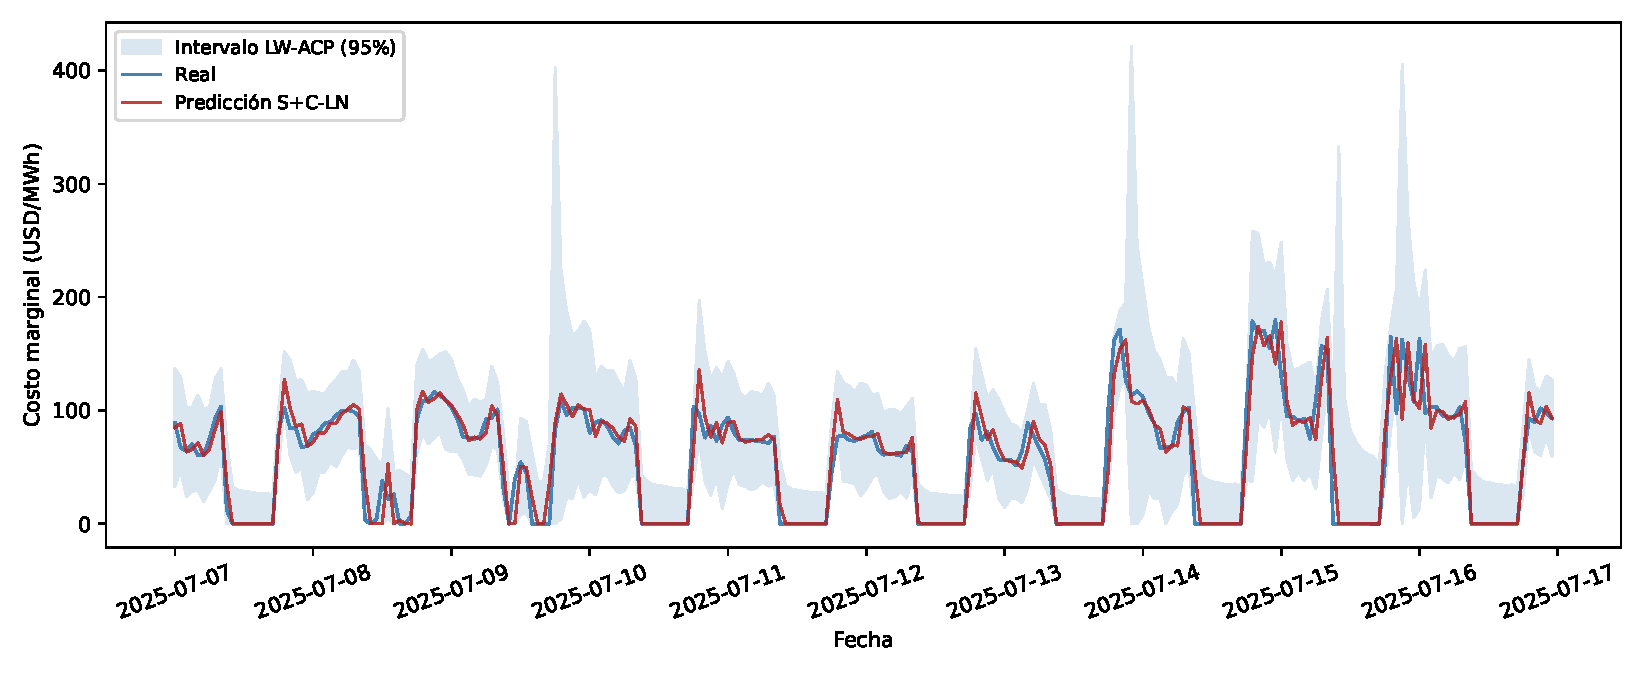
\includegraphics[width=0.75\textwidth]{imagenes/fig_cp_ejemplo_intervalo.pdf}
    \caption{Ejemplo de intervalo de predicción LW-ACP (95\% nominal) para Atacama, 12 de febrero de 2026. El intervalo se angosta en las horas de precio cero (mediodía, sobreoferta solar) y se ensancha en las horas de transición, capturando correctamente el \textit{peak} matutino sin dejar de ser informativo.}
    \label{fig:cp_ejemplo_intervalo}
\end{figure}

\subsection{Split CP clásico}
\label{sec:split_cp_clasico}

Consistente con la selección de S+C-LN como modelo de referencia para el resto de este capítulo (Sección \ref{sec:pc_vs_sc}), el Split CP clásico se construye directamente sobre la predicción cruda del $\text{TFT}_\text{LN}$ S+C, sin pasar por Stacking Optimization: no existe una combinación de múltiples predicciones con pesos aprendidos, por lo que no hay una columna de ``estrategia'' que varíe entre barras. Los resultados se presentan en la Tabla \ref{tab:scp_resultados}.

\begin{table}[htbp]
    \centering
    \small
    \begin{tabular}{lrrrr}
        \toprule
        Barra & Coverage & Width & MAE & $q$ \\
        \midrule
        Atacama       & 0.9648 & 54.68  & 6.70  & 34.07 \\
        Cardones      & 0.9595 & 53.58  & 6.63  & 33.25 \\
        Charrúa       & 0.9512 & 61.23  & 7.98  & 35.51 \\
        Crucero       & 0.9614 & 52.82  & 6.74  & 32.90 \\
        Pan de Azúcar & 0.9588 & 57.16  & 6.93  & 35.38 \\
        Puerto Montt  & 0.9600 & 110.41 & 13.68 & 64.05 \\
        Quillota      & 0.9530 & 64.25  & 8.26  & 37.43 \\
        Tarapacá      & 0.9623 & 56.23  & 7.11  & 35.24 \\
        \bottomrule
    \end{tabular}
    \caption{Resultados del Split CP clásico sobre S+C-LN, las ocho barras del SEN. Coverage nominal: 0.95. Width, MAE y $q$ en USD/MWh. El límite inferior de todos los intervalos se trunca en 0 USD/MWh, respetando el dominio físico del costo marginal; $q$ es el semiancho antes de truncar.}
    \label{tab:scp_resultados}
\end{table}

Los resultados muestran cobertura empírica por encima del nominal en las ocho barras. La cobertura oscila entre 0.9512 (Charrúa) y 0.9648 (Atacama), con anchos medios entre 52.8 (Crucero) y 64.3 USD/MWh (Quillota) en las siete barras del norte y centro, y un ancho considerablemente mayor en Puerto Montt (110.4 USD/MWh), consistente con su mayor dispersión de precio ya documentada en la Sección \ref{sec:pmontt_desempeno}. El caso de Charrúa es especialmente relevante: es la barra que más se acerca al nominal exacto, con una diferencia de cobertura de apenas 0.12 puntos porcentuales, consistente con que Charrúa es también la barra donde el TFT S+C tiene mayor MAE relativo entre las siete barras del norte y centro, lo que produce errores de calibración más representativos del comportamiento en prueba.

El ancho reportado en esta y las siguientes tablas de esta sección ya incorpora el truncamiento en 0 del límite inferior del intervalo, aplicado de manera uniforme a los cinco métodos (Split CP, ACI, LW Split CP, LW-ACP y CQR): dado que el costo marginal no toma valores negativos, un límite inferior negativo no aporta información y solo infla artificialmente el ancho reportado, sobre todo en horas de precio cercano a cero. El truncamiento no afecta la cobertura empírica --un intervalo $[\hat{y}-q, \hat{y}+q]$ con $\hat y - q<0$ cubre $y\geq 0$ exactamente cuando $[\max(\hat y-q,0), \hat y+q]$ también lo cubre--, por lo que las cifras de cobertura de esta sección son idénticas con o sin truncar; el efecto es puramente una reducción del ancho medio, más marcada cuanto más frecuentes son las horas de precio bajo en la barra.

La sobrecobertura observada en Atacama, de hasta 1.5 puntos porcentuales sobre el nominal, es el efecto esperado de un cuantil fijo calculado sobre el período de validación: si la distribución de errores en prueba es más concentrada que en calibración, el intervalo resulta conservadoramente ancho. Esta limitación motiva las variantes adaptativas.

Como se detalla en la Sección \ref{sec:cp_configuracion_general} del Marco Metodológico, la calibración de los cinco métodos de esta sección excluye una ventana de 11 horas de precio de falla administrativo (25--26 de febrero de 2025), verificada por el mismo valor exacto simultáneo en las ocho barras. Esta ventana cae en el conjunto de validación (calibración), no en prueba, por lo que no afecta directamente el MAE de prueba reportado en el resto de este capítulo, pero sí inflaba el cuantil de no conformidad antes de excluirla.

\subsection{ACI}
\label{sec:aci}

A diferencia de una formulación anterior de este trabajo, que construía un meta-modelo Ridge auxiliar (predicción de S+C-LN más las variables solares \texttt{elevacion\_solar} y \texttt{cos\_elevacion}) como predictor puntual para ACI, aquí ACI se evalúa sobre la misma predicción cruda de S+C-LN que Split CP, LW Split CP y LW-ACP: usar un predictor distinto por método impediría comparar el ancho de intervalo entre ellos de forma válida (Sección \ref{sec:lwacp_comparativa}), ya que el efecto del mecanismo de calibración quedaría mezclado con el efecto de cambiar el modelo base. Al no requerir ningún meta-modelo, ACI tampoco distingue entre una variante \textit{offline} y una \textit{online} --la distinción original aludía a si el meta-modelo se reajustaba en cada paso de prueba, algo que ya no aplica-- por lo que se reporta un único método. Se fija $\gamma = 0.05$ de antemano, el mismo valor usado en LW-ACP (Sección \ref{sec:lwacp_resultados}), en lugar de comparar varios valores de $\gamma$ y reportar el de mejor desempeño en prueba. Los resultados se presentan en la Tabla \ref{tab:aci_ln_resultados}.

\begin{table}[htbp]
    \centering
    \small
    \begin{tabular}{lrrrr}
        \toprule
        Barra & Coverage & Width & MAE & $\bar{\alpha}_t$ \\
        \midrule
        Atacama       & 0.9467 & 49.72  & 6.70  & 0.0878 \\
        Cardones      & 0.9465 & 47.14  & 6.63  & 0.0903 \\
        Charrúa       & 0.9443 & 57.14  & 7.98  & 0.0825 \\
        Crucero       & 0.9469 & 49.58  & 6.74  & 0.0890 \\
        Pan de Azúcar & 0.9461 & 49.32  & 6.93  & 0.0905 \\
        Puerto Montt  & 0.9471 & 105.71 & 13.68 & 0.0841 \\
        Quillota      & 0.9446 & 58.09  & 8.26  & 0.0818 \\
        Tarapacá      & 0.9472 & 52.88  & 7.11  & 0.0876 \\
        \bottomrule
    \end{tabular}
    \caption{Resultados de ACI sobre S+C-LN (predictor puntual crudo, sin meta-modelo) con $\gamma = 0.05$ fijo, las ocho barras del SEN. Coverage nominal: 0.95. Width y MAE en USD/MWh. $\bar{\alpha}_t$: media temporal del nivel adaptado.}
    \label{tab:aci_ln_resultados}
\end{table}

Dos patrones emergen de los resultados. Primero, la cobertura empírica se mantiene cercana al nominal en las ocho barras, con errores de cobertura entre 0.28 (Tarapacá) y 0.57 puntos porcentuales (Charrúa) --sensiblemente mejor que la sobrecobertura de 0.9--1.5 puntos de Split CP (Sección \ref{sec:split_cp_clasico})--, confirmando que la adaptación \textit{online} de $\alpha_t$ corrige el sesgo de sobrecobertura estructural del cuantil fijo. Segundo, y a diferencia de una lectura anterior de este mismo análisis --hecha antes de excluir de la calibración la ventana de precio de falla administrativo (Sección \ref{sec:split_cp_clasico})--, el ancho de intervalo de ACI \textbf{sí es sistemáticamente menor} que el de Split CP una vez que ambos comparten el mismo predictor puntual: el ancho promedio de ACI (58.7\,USD/MWh) es 8.0\% menor que el de Split CP (63.8), con una reducción que va de 4.3\% (Puerto Montt) a 13.7\% (Pan de Azúcar). El cuantil de no conformidad de un método de cuantil fijo como Split CP es especialmente sensible a un puñado de \textit{scores} de calibración inflados por un evento no representativo del mercado; la adaptación \textit{online} de $\alpha_t$, al recalcularse en cada paso de prueba en vez de fijarse una sola vez, resulta menos expuesta a ese mismo sesgo. El aporte de ACI, medido correctamente, es entonces doble: mejor calibración y un intervalo más angosto, no solo lo primero.

\subsection{LW Split CP}
\label{sec:lw_split_cp}

Al igual que Split CP clásico y ACI (Secciones \ref{sec:split_cp_clasico}--\ref{sec:aci}), LW Split CP y LW-ACP (Sección \ref{sec:lwacp_resultados}) se evalúan sobre S+C-LN, manteniendo la misma arquitectura, rama y predictor puntual en las ocho barras. La Tabla \ref{tab:lwscp_resultados} presenta los resultados de LW Split CP.

\begin{table}[htbp]
    \centering
    \small
    \begin{tabular}{lrrr}
        \toprule
        Barra & Coverage & Width & MAE \\
        \midrule
        Atacama       & 0.9651 & 55.80  & 6.70  \\
        Cardones      & 0.9588 & 54.19  & 6.63  \\
        Charrúa       & 0.9537 & 61.79  & 7.98  \\
        Crucero       & 0.9623 & 53.76  & 6.74  \\
        Pan de Azúcar & 0.9601 & 56.75  & 6.93  \\
        Puerto Montt  & 0.9597 & 109.53 & 13.68 \\
        Quillota      & 0.9535 & 62.98  & 8.26  \\
        Tarapacá      & 0.9612 & 56.67  & 7.11  \\
        \bottomrule
    \end{tabular}
    \caption{Resultados de LW Split CP sobre S+C-LN, las ocho barras del SEN. Coverage nominal: 0.95. Width y MAE en USD/MWh.}
    \label{tab:lwscp_resultados}
\end{table}

La cobertura empírica se mantiene por encima del nominal en las ocho barras, entre 0.9535 (Quillota) y 0.9651 (Atacama), un patrón de sobrecobertura similar al de Split CP clásico (Sección \ref{sec:split_cp_clasico}) y esperable dado que LW Split CP hereda el mismo mecanismo de cuantil fijo, solo que aplicado sobre \textit{scores} normalizados por hora. El ancho medio, sin embargo, \textbf{no se reduce de forma consistente} respecto a Split CP clásico: sube en Atacama (+2.1\%), Cardones (+1.1\%), Charrúa (+0.9\%), Crucero (+1.8\%) y Tarapacá (+0.8\%), y baja levemente en Pan de Azúcar (-0.7\%), Puerto Montt (-0.8\%) y Quillota (-2.0\%), sin una dirección predominante (63.9 vs.\ 63.8\,USD/MWh en promedio sobre las ocho barras, +0.2\%). Esto contrasta con ACI (Sección \ref{sec:aci}), que sí reduce el ancho de forma sistemática y por un margen considerable (8.0\%): la ponderación local por hora, aplicada sola y sin la adaptación \textit{online} de $\alpha_t$, no es suficiente para capturar una ganancia de eficiencia -- la Sección \ref{sec:lwacp_comparativa} retoma esta comparación con los cinco métodos en conjunto.

\subsection{LW-ACP Online}
\label{sec:lwacp_resultados}

La Tabla \ref{tab:lwacp_resultados} presenta los resultados de LW-ACP sobre S+C-LN, la variante que combina la ponderación local por hora con la actualización online del nivel de cobertura de ACI (Sección \ref{sec:lwacp}), con $\gamma = 0.05$ fijo, el mismo valor usado en ACI (Sección \ref{sec:aci}) y no seleccionado comparando contra el resultado en prueba.

\begin{table}[htbp]
    \centering
    \small
    \begin{tabular}{lrrr}
        \toprule
        Barra & Coverage & Width & MAE \\
        \midrule
        Atacama       & 0.9471 & 49.62  & 6.70  \\
        Cardones      & 0.9461 & 48.47  & 6.63  \\
        Charrúa       & 0.9440 & 56.29  & 7.98  \\
        Crucero       & 0.9471 & 49.99  & 6.74  \\
        Pan de Azúcar & 0.9461 & 48.96  & 6.93  \\
        Puerto Montt  & 0.9475 & 101.34 & 13.68 \\
        Quillota      & 0.9440 & 58.04  & 8.26  \\
        Tarapacá      & 0.9476 & 53.33  & 7.11  \\
        \bottomrule
    \end{tabular}
    \caption{Resultados de LW-ACP ($\gamma = 0.05$) sobre S+C-LN, las ocho barras del SEN. Coverage nominal: 0.95. Width y MAE en USD/MWh.}
    \label{tab:lwacp_resultados}
\end{table}

La cobertura empírica de LW-ACP se mantiene cerca del nominal: las ocho barras caen en el rango $[0.9440,\, 0.9476]$, es decir, entre 0.24 y 0.60 puntos porcentuales del nominal 0.95, más ajustado que la sobrecobertura de 0.1--1.5 puntos porcentuales observada en Split CP clásico y LW Split CP, aunque sin la precisión casi exacta que se obtenía con $\gamma = 0.01$ --el valor con el que se había barrido inicialmente, y que producía una desviación media de solo 0.02 puntos porcentuales, pero que no puede adoptarse sin verse influido por su desempeño en prueba (Sección \ref{sec:lwacp_comparativa})--. Esto confirma que el mecanismo de adaptación online de $\alpha_t$, heredado de ACI, corrige de manera efectiva el sesgo de sobrecobertura estructural de los métodos de cuantil fijo, sin necesidad de reentrenar ningún modelo, aunque la magnitud exacta de esa corrección depende de $\gamma$.

Al mismo tiempo, LW-ACP produce los intervalos más angostos de los cinco métodos evaluados, incluyendo CQR como comparación externa (Sección \ref{sec:lwacp_comparativa}): una reducción promedio de 8.7\% respecto a Split CP clásico, con el mayor beneficio en Pan de Azúcar (14.4\%) y Cardones (9.5\%), y el menor en Tarapacá (5.2\%) y Crucero (5.4\%). La mayor parte de esta reducción ya está presente en ACI solo (8.0\% respecto a Split CP, Sección \ref{sec:aci}); la ponderación local por hora, agregada sobre la adaptación \textit{online}, aporta una reducción adicional modesta (LW-ACP es 0.8\% más angosto que ACI en promedio) pero no uniforme, angosto en cinco de las ocho barras y levemente más ancho en las otras tres (Cardones, Crucero, Tarapacá). La combinación de una cobertura cercana al nominal y el ancho más angosto de los cinco métodos muestra que, con un $\gamma$ fijado de antemano y no elegido por su resultado en prueba, LW-ACP explota dos fuentes de información distintas --la heterocedasticidad horaria conocida de antemano, vía $\hat{\sigma}_h$, y el error de cobertura reciente, vía $\alpha_t$--, aunque la segunda explica la mayor parte de la ganancia y la primera aporta un refinamiento adicional, no una fuente de eficiencia comparable por sí sola (Sección \ref{sec:lw_split_cp}).

\subsection{Comparativa de métodos: SCP, ACP, LW-ACP y CQR}
\label{sec:lwacp_comparativa}

Con todos los métodos evaluados sobre S+C-LN y sobre el mismo predictor puntual crudo, las tres variantes principales de Split CP forman un linaje conceptual de dos pasos, más una comparación externa: Split CP (SCP) es el método base de calibración por cuantil fijo (Sección \ref{sec:split_cp_clasico}); ACP añade adaptación \textit{online} del nivel de cobertura, el mecanismo de Gibbs y Candès (2021, Sección 2.6.4), correspondiente a ACI con $\gamma = 0.05$ (Sección \ref{sec:aci}); y LW-ACP, la contribución de este trabajo, añade además ponderación local por hora (Sección \ref{sec:lwacp_resultados}, Sección \ref{sec:lwacp} del Marco Teórico). CQR se incluye como comparación externa a la familia de Conformal Prediction (Sección 2.6.2), al estimar cuantiles condicionales directamente mediante regresión cuantílica en vez de calibrar un cuantil de no conformidad. La Tabla \ref{tab:lw_comparativa} resume el ancho medio, la desviación de cobertura y el \textit{interval score} de Winkler --que penaliza conjuntamente el ancho del intervalo y la magnitud de la no-cobertura, a diferencia del ancho y la cobertura marginal por separado (Sección \ref{sec:metricas_cp})-- de los cuatro métodos, promediados sobre las ocho barras.

\begin{table}[htbp]
    \centering
    \begin{tabular}{lrrr}
        \toprule
        Método & Width medio (USD/MWh) & $|$Coverage $-$ 0.95$|$ medio & Winkler medio \\
        \midrule
        Split CP (SCP)              & 63.80 & 0.0089 & 100.78 \\
        ACP (ACI, $\gamma=0.05$)    & 58.70 & 0.0038 & 90.64 \\
        LW-ACP ($\gamma=0.05$)      & \textbf{58.25} & \textbf{0.0038} & \textbf{89.89} \\
        CQR                         & 67.99 & 0.0081 & 96.50 \\
        \bottomrule
    \end{tabular}
    \caption{Comparación del linaje SCP $\to$ ACP $\to$ LW-ACP, más CQR como comparación externa, evaluados sobre S+C-LN con el mismo predictor puntual crudo (ocho barras). Width y Winkler promedio en USD/MWh; desviación absoluta media respecto a la cobertura nominal 0.95.}
    \label{tab:lw_comparativa}
\end{table}

El linaje SCP $\to$ ACP $\to$ LW-ACP, con $\gamma = 0.05$ fijado de antemano y el mismo predictor puntual crudo en los tres métodos, muestra que casi toda la ganancia del linaje proviene de un solo mecanismo. ACP, que solo añade adaptación \textit{online} del nivel de cobertura, sin ponderación horaria ni cambio de predictor, reduce la desviación de cobertura en 57\% (de 0.0089 a 0.0038 puntos) respecto a SCP, y \textbf{también reduce el ancho medio} de forma sustancial: con 58.70\,USD/MWh resulta 8.0\% más angosto que SCP (Sección \ref{sec:aci}). LW-ACP, que agrega la ponderación por hora sobre ese mismo mecanismo \textit{online}, reduce el ancho un poco más, hasta 58.25\,USD/MWh (8.7\% respecto a SCP), con una calibración prácticamente idéntica a la de ACP solo (0.0038 en ambos). En conjunto, esto acota con precisión qué aporta cada mecanismo, y corrige una lectura anterior de este mismo análisis: la adaptación \textit{online} de $\alpha_t$ por sí sola ya explica la gran mayoría de la mejora, tanto en calibración como en ancho; la ponderación horaria por sí sola, sin adaptación \textit{online}, no aporta una reducción de ancho consistente (Sección \ref{sec:lw_split_cp}), y solo aporta un refinamiento adicional modesto cuando se combina con la adaptación \textit{online} en LW-ACP. CQR, evaluado de forma independiente de la familia CP, resulta en este caso el \textbf{más ancho} de los cuatro métodos (67.99\,USD/MWh) y con peor calibración que ACP y LW-ACP (0.0081 de desviación, más del doble): a diferencia de los tres métodos conformes, cuyo intervalo se trunca en 0 de forma directa sobre un semiancho ya angosto, los cuantiles de CQR se estiman por regresión cuantílica condicional y ya incorporan una asimetría propia que deja menos margen para que el truncamiento en 0 reduzca su ancho reportado. El \textit{interval score} de Winkler, que combina ambas dimensiones en una sola métrica, confirma este orden (LW-ACP $<$ ACP $<$ CQR $<$ SCP): LW-ACP obtiene el mejor puntaje (89.89), seguido de cerca por ACP (90.64), con CQR intermedio (96.50) y SCP claramente peor (100.78, 12\% más alto que LW-ACP). LW-ACP es entonces el único de los cuatro métodos que combina el mejor resultado en las tres métricas --ancho, calibración y Winkler-- de forma simultánea.

Queda fuera de esta comparación agregada, aunque se presenta en su propia sección, LW Split CP (Sección \ref{sec:lw_split_cp}), que pondera por hora sin adaptación \textit{online}: confirma, desde la dirección opuesta a ACP, que la ponderación horaria por sí sola no es la fuente principal de la eficiencia observada en LW-ACP.

\subsection{Cobertura condicional por hora y por mes}
\label{sec:cobertura_condicional}

La cobertura marginal cercana al nominal reportada hasta aquí es un promedio sobre todo el conjunto de prueba, y puede ocultar heterogeneidad sistemática si el método sub-cubre en algunas horas o meses y sobre-cubre en otras, compensándose en el promedio. Esta sección desagrega la cobertura de Split CP, ACP y LW-ACP --el linaje completo (Sección \ref{sec:lwacp_comparativa})-- por hora del día y por mes, promediando sobre las ocho barras.

La Figura \ref{fig:cp_cobertura_ancho_hora} presenta la cobertura y el ancho medio por hora del día para los tres métodos. Incluir a ACP, no solo los dos extremos del linaje, permite distinguir si la caída de cobertura en horas de transición es un efecto de la adaptación \textit{online} en sí, o específico de agregarle la ponderación horaria: la Figura \ref{fig:cp_cobertura_ancho_hora} muestra que ACP y LW-ACP caen de forma casi idéntica en esas horas (0.902 vs.\ 0.898), mientras que Split CP, sin adaptación \textit{online}, cae menos (0.943). La caída es entonces atribuible al mecanismo de adaptación \textit{online} de $\alpha_t$, compartido por ambos métodos, no a la ponderación horaria que solo LW-ACP incorpora.

\begin{figure}[htbp]
    \centering
    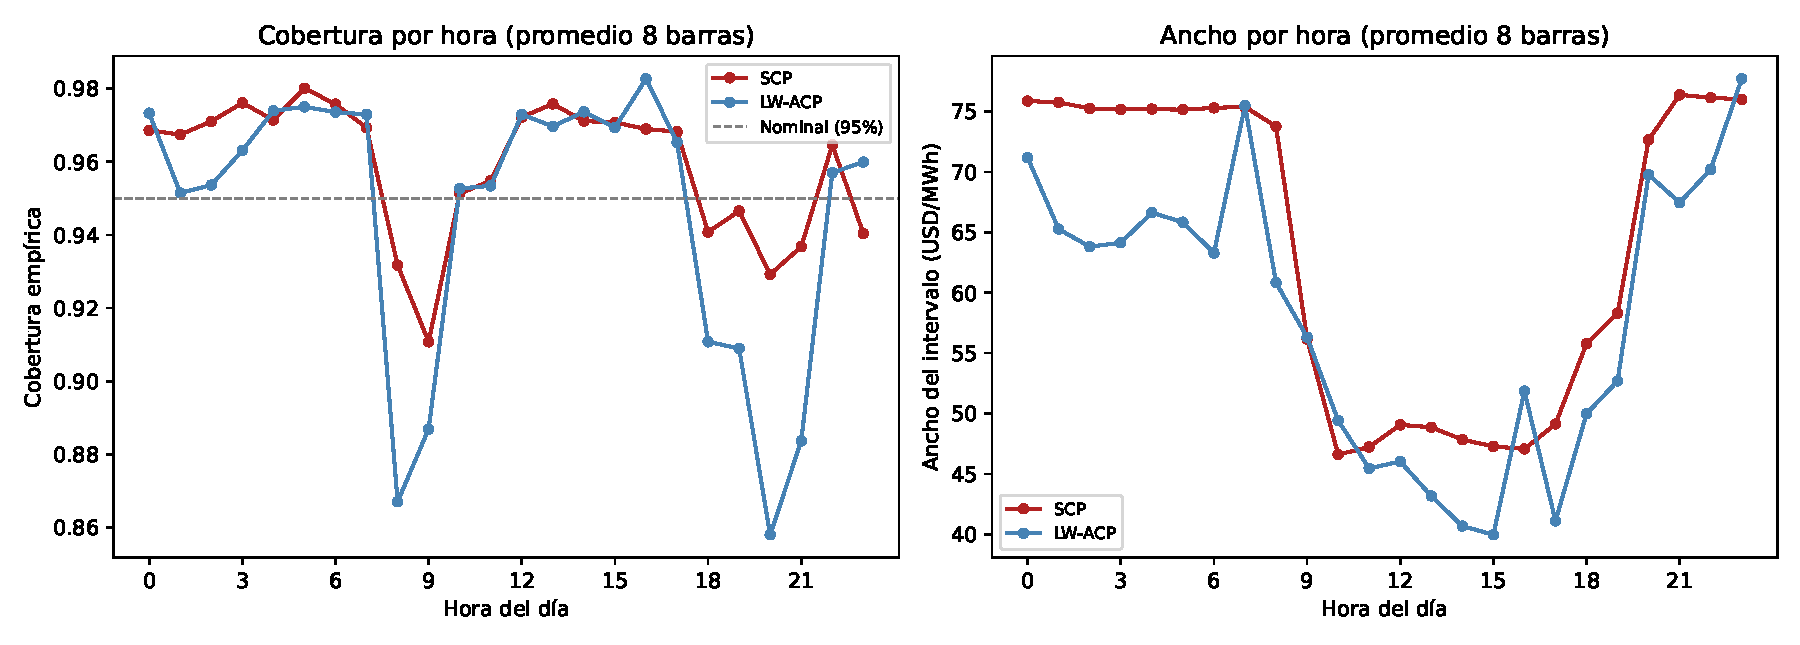
\includegraphics[width=\textwidth]{imagenes/fig_cp_cobertura_ancho_hora.pdf}
    \caption{Cobertura empírica (izquierda) y ancho medio del intervalo (derecha) por hora del día, Split CP vs.\ ACP vs.\ LW-ACP, promediado sobre las ocho barras. ACP y LW-ACP son más angostos que Split CP casi todo el día, pero ambos --no solo LW-ACP-- caen marcadamente por debajo del nominal en las horas de transición solar (7--9h, 19--21h).}
    \label{fig:cp_cobertura_ancho_hora}
\end{figure}

Por mes, LW-ACP es marcadamente más estable que Split CP: la desviación estándar de la cobertura mensual es 0.0048 para LW-ACP frente a 0.0280 para Split CP, casi seis veces menor. Split CP oscila entre 0.899 (junio) y 0.991 (marzo), mientras que las doce cifras mensuales de LW-ACP caen todas en el rango estrecho $[0.933,\, 0.950]$. Esta es precisamente la ventaja esperada de la adaptación \textit{online} de $\alpha_t$: al reaccionar al historial reciente de cobertura, LW-ACP corrige la deriva estacional que un cuantil fijo como el de Split CP no puede seguir.

Por hora del día, sin embargo, el resultado es el opuesto: la desviación estándar de la cobertura horaria es 0.0181 para Split CP frente a 0.0370 para LW-ACP, más del doble. La brecha se concentra exactamente en las horas de transición solar (7, 8, 19, 20 y 21h) que el análisis de errores extremos (Sección \ref{sec:errores_extremos}) ya identifica como el origen del desfase de fase: ahí la cobertura promedio de LW-ACP cae a 0.898, 5.2 puntos porcentuales bajo el nominal y 4.5 puntos por debajo de Split CP (0.943) en esas mismas horas, mientras que en el resto de las horas ambos métodos son similares (0.959 LW-ACP vs.\ 0.963 Split CP). Es decir, la ponderación horaria por sí sola no logra homogeneizar la cobertura entre horas --la motivación original de $\hat\sigma_h$--, y en las horas más difíciles del día, las mismas donde se concentra el desfase de fase, LW-ACP cubre peor que el cuantil fijo sin ponderar, no mejor.

Esto es coherente con el hallazgo de la Sección \ref{sec:lwacp_comparativa}: la eficiencia de LW-ACP proviene mayoritariamente de la adaptación \textit{online} de $\alpha_t$, un mecanismo que opera sobre la dimensión temporal mes a mes, no sobre la dimensión horaria intradía. $\hat\sigma_h$ ajusta el \textit{ancho} del intervalo según la variabilidad histórica de cada hora, pero no ajusta el \textit{nivel de cobertura} por hora --ese es un único $\alpha_t$ compartido por las 24 horas del día--, por lo que un error sistemático concentrado en horas específicas, como el desfase de fase, no se corrige de la misma forma en que la adaptación \textit{online} sí corrige la deriva estacional. Esta limitación motiva directamente la variante de $\alpha_t$ indexado por hora propuesta como trabajo futuro (Conclusiones).

\subsection{Selección del mejor método de CP}

LW-ACP es el método de Conformal Prediction seleccionado para el pipeline final. Es el único de los cuatro métodos que combina el mejor resultado en las tres métricas evaluadas: el ancho medio más angosto (58.25\,USD/MWh, 8.7\% menor que Split CP), la mejor calibración (0.0038 de desviación media, empatado con ACP y menos de la mitad de la desviación de CQR) y el mejor \textit{interval score} de Winkler (89.89, Sección \ref{sec:lwacp_comparativa}), dentro de 0.24--0.60 puntos porcentuales del nominal en las ocho barras (Sección \ref{sec:lwacp_resultados}). A diferencia de CQR, que no ofrece garantías de cobertura marginal finita sin supuestos distribucionales y que en esta comparación resulta ser el método más ancho de los cuatro, LW-ACP hereda la garantía de cobertura marginal asintótica de la familia conforme, y logra además reducir el ancho respecto a Split CP en las ocho barras sin excepción (Sección \ref{sec:lwacp_resultados}). Esta ventaja en ancho proviene principalmente de la adaptación \textit{online} del nivel de cobertura, heredada de ACP, con un aporte adicional --menor, y consistente en cinco de las ocho barras-- de la ponderación horaria vía $\hat{\sigma}_h$ (Sección \ref{sec:lwacp_comparativa}).

La cobertura condicional (Sección \ref{sec:cobertura_condicional}) matiza esta elección sin invalidarla: LW-ACP es notablemente más estable que Split CP mes a mes, pero menos uniforme hora a hora, con una brecha de cobertura concreta en las horas de transición solar donde se concentra el desfase de fase. La elección de LW-ACP se sostiene en su desempeño marginal --ancho, calibración y Winkler score-- y en su estabilidad temporal frente a la deriva estacional, no en haber resuelto la heterogeneidad horaria del error, que sigue siendo una limitación abierta.

Cabe señalar una limitación metodológica del diseño experimental: el conjunto de validación cumple simultáneamente el rol de selección del mejor ensamble y de calibración del CP, lo que introduce un sesgo optimista en el cuantil de no conformidad. Este sesgo es esperablemente pequeño dado el tamaño del conjunto de calibración ($n_{\text{cal}} = 8\,298$) y la estabilidad de los residuos del ensamble, pero se reporta para transparencia metodológica.

\subsection{Análisis de errores extremos}
\label{sec:errores_extremos}

La brecha entre el MAE promedio del modelo (6.89\,USD/MWh en validación para Atacama) y el semiancho de los intervalos de Split CP clásico ($q = 32.72$\,USD/MWh, Sección \ref{sec:split_cp_clasico}) sugiere que la distribución de errores del modelo no es simétrica ni de cola ligera. Para comprender el origen de esta brecha, se examina la distribución de errores absolutos en validación para las ocho barras, con Atacama como caso ilustrativo y el detalle completo del resto en el Anexo \ref{anexo:errores_extremos}.

La Figura \ref{fig:error_dist_atacama} muestra la distribución de
errores absolutos del $\text{TFT}_\text{LN}$ (S+C) en validación para Atacama. La distribución presenta una forma exponencial decreciente fuertemente concentrada: más del 90\% de las predicciones tienen un error menor a 19.8\,USD/MWh, y el percentil 95 es de 32.5\,USD/MWh. Sin embargo, la distribución exhibe una cola derecha extendida que alcanza los 162.9\,USD/MWh, marcada explícitamente en la figura. Es precisamente esta cola la que determina el cuantil de calibración del Split CP: $q = 32.72$\,USD/MWh corresponde aproximadamente al percentil 95 de la distribución de errores de validación, de modo que el ancho del intervalo queda dominado por el 5\% de los errores más grandes. Las ocho barras exhiben la misma forma general, con el máximo desplazándose entre 132.4 (Charrúa) y 241.7\,USD/MWh (Puerto Montt); ver Anexo \ref{anexo:errores_extremos} para el detalle de errores por barra.

\begin{figure}[htbp]
    \centering
    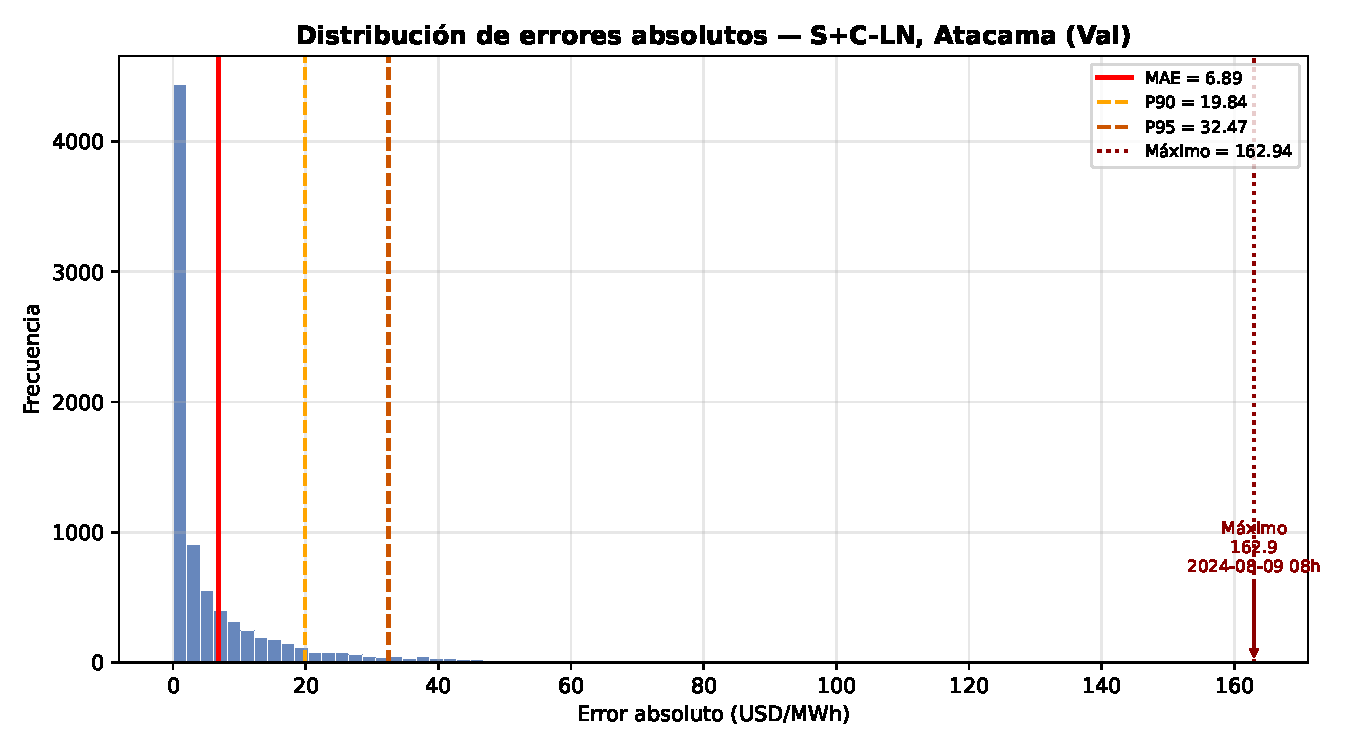
\includegraphics[width=0.95\textwidth]{imagenes/fig_error_dist_atacama.pdf}
    \caption{Distribución de errores absolutos del $\text{TFT}_\text{LN}$ (S+C)
    en el conjunto de validación para la barra Atacama ($n = 8\,298$ observaciones).  Las líneas verticales indican el MAE (rojo), el percentil 90 (naranja claro), el percentil 95 (naranja oscuro) y el error máximo (granate, punteado), este último señalado además con una flecha dado lo alejado que queda del grueso de la distribución.}
    \label{fig:error_dist_atacama}
\end{figure}

Una primera hipótesis ante una cola de este tipo es que los errores
extremos correspondan a eventos inusuales de la propia serie temporal: spikes de costo marginal asociados a indisponibilidades, eventos climáticos o cambios regulatorios que el modelo no puede anticipar por construcción, dado que no dispone de información futura sobre dichos eventos. Bajo esa hipótesis, los errores grandes serían inherentes a la naturaleza del problema y no reflejarían una deficiencia del modelo. Para evaluar esta hipótesis, se examinan en detalle los 20 errores absolutos más grandes del conjunto de validación de cada barra: se recalcula el error tras desplazar la predicción entre $-3$ y $+3$ horas respecto de su posición original, y se retiene el desplazamiento que minimiza el error resultante; si la reducción de error alcanzada supera el 60\%, el caso se clasifica como \textit{desfase de fase}, y como \textit{evento estructural} en caso contrario. El Anexo \ref{anexo:errores_extremos} presenta la tabla completa de los 20 mayores errores para cada barra; la Tabla \ref{tab:sintesis_errores} resume los resultados a nivel de todo el SEN.

\begin{table}[htbp]
    \centering
    \small
    \begin{tabular}{lrrrrr}
        \toprule
        Barra & MAE & P95 & Máximo & Desfase de fase & Transición solar \\
        \midrule
        Atacama       & 6.89  & 32.47 & 162.94 & 17/20 & 12/20 \\
        Cardones      & 6.91  & 32.15 & 164.48 & 17/20 & 11/20 \\
        Charrúa       & 7.78  & 35.18 & 132.36 & 17/20 &  9/20 \\
        Crucero       & 6.95  & 31.46 & 174.38 & 18/20 & 13/20 \\
        Pan de Azúcar & 7.41  & 35.07 & 143.70 & 17/20 & 10/20 \\
        Puerto Montt  & 14.97 & 63.83 & 241.73 & 20/20 &  1/20 \\
        Quillota      & 7.98  & 37.05 & 144.20 & 16/20 &  8/20 \\
        Tarapacá      & 7.36  & 33.21 & 169.64 & 17/20 & 15/20 \\
        \bottomrule
    \end{tabular}
    \vspace{0.2cm}
    \caption{Síntesis del análisis de errores extremos en validación, las ocho barras del SEN. MAE, P95 y Máximo en USD/MWh. \textit{Desfase de fase}: cuántos de los 20 mayores errores se clasifican como tal (vs.\ \textit{evento estructural}). \textit{Transición solar}: cuántos de los 20 ocurren en las horas 07:00--08:00 o 19:00--21:00. Detalle completo por barra en el Anexo \ref{anexo:errores_extremos}.}
    \label{tab:sintesis_errores}
\end{table}

El análisis cuantitativo descarta en gran medida la hipótesis de
eventos inusuales en la serie: en las ocho barras, entre el 80\% y el 100\% de los 20 mayores errores corresponden a un \textit{desfase de fase} y no a spikes anómalos del costo marginal, con una reducción de error mediana entre el 84\% y el 98\% al desplazar la predicción (típicamente 1 hora, ocasionalmente 2). El sentido del desplazamiento es sistemáticamente el mismo en las ocho barras: entre el 76\% y el 94\% de los casos de desfase requieren un desplazamiento positivo, es decir, \textbf{el modelo predice la transición del costo marginal con un retraso aproximado de una hora respecto a la transición real}, un patrón consistente en todo el SEN y no un artefacto de una barra particular.

Puerto Montt es la excepción que confirma la regla: sus 20 mayores errores se clasifican \emph{todos} como desfase de fase (reducción mediana del 98\%, la más alta del grupo), pero solo 1 de 20 ocurre en las horas de transición solar 07:00--08:00 o 19:00--21:00, frente a 8--15 de 20 en las siete barras restantes. Esto es consistente con el resto de la caracterización de Puerto Montt en este capítulo (Sección \ref{sec:pmontt_desempeno}): el desfase de fase es un patrón general del modelo, no específico del ciclo solar, y en Puerto Montt se manifiesta alrededor de la dinámica hidrológica de la zona en vez de las transiciones de amanecer/atardecer.

La Figura \ref{fig:phase_shift_panel} ilustra cuatro casos
representativos de Atacama: tres desfases de fase en transiciones de amanecer o atardecer, y un evento estructural, un spike abrupto en la serie real que el modelo suaviza, consistente con un evento de indisponibilidad o redespacho no capturado por las covariables disponibles. Los paneles equivalentes para las siete barras restantes se presentan en el Anexo \ref{anexo:errores_extremos}.

\begin{figure}[htbp]
    \centering
    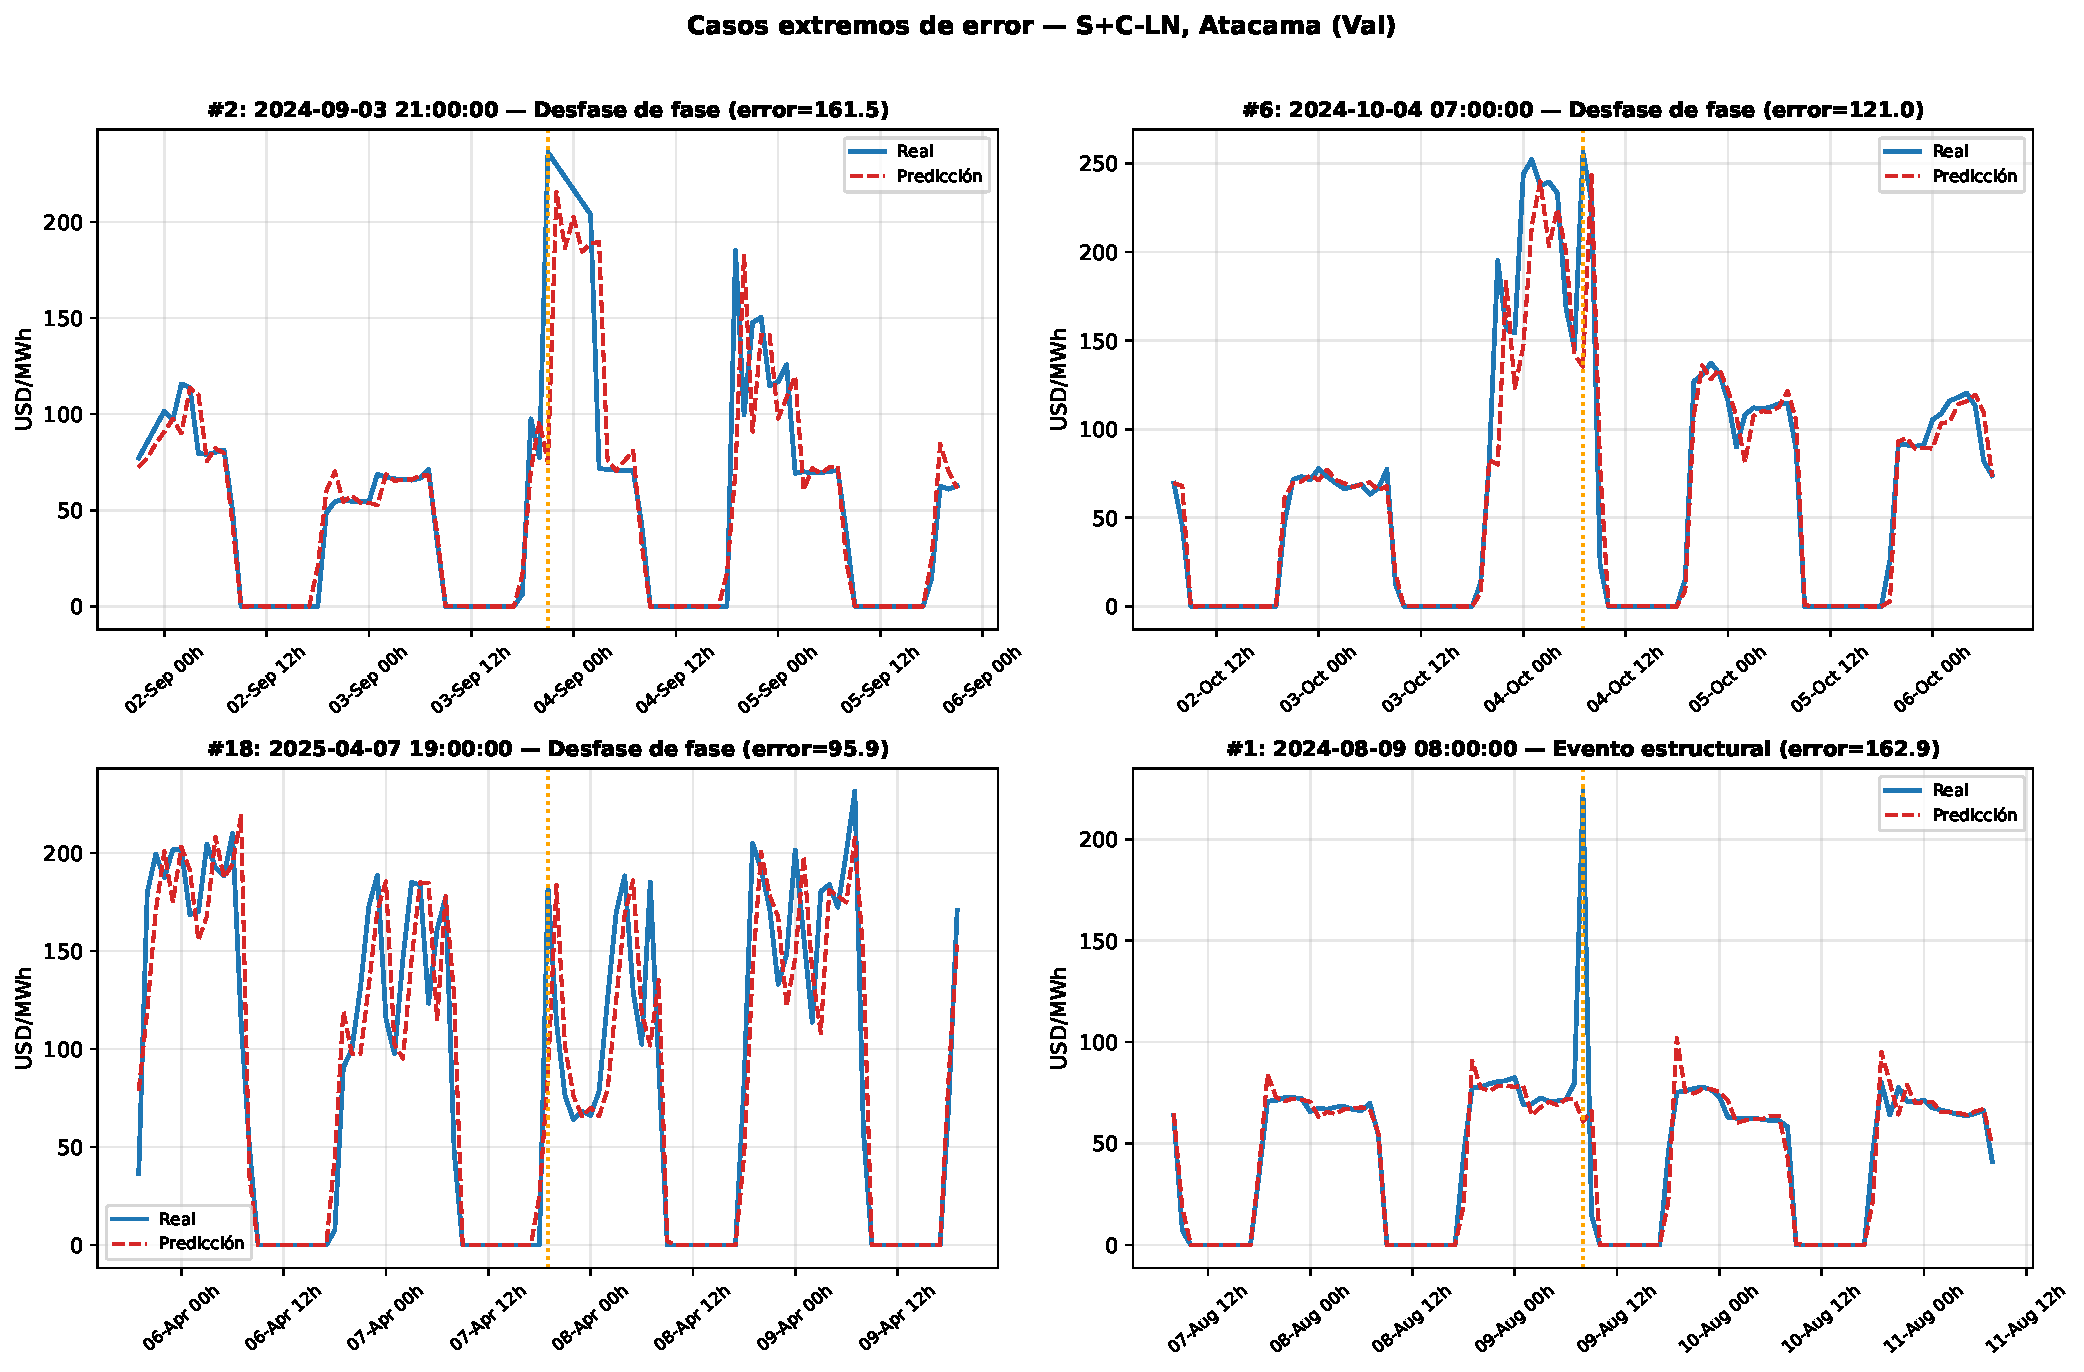
\includegraphics[width=\textwidth]{imagenes/fig_phase_shift_panel_2x2.pdf}
    \caption{Casos extremos de error del $\text{TFT}_\text{LN}$ (S+C) para
    la barra Atacama en validación.  Cada panel muestra una ventana de
    $\pm$48\,h alrededor del instante de error máximo (línea vertical
    punteada naranja).  La curva azul corresponde al CMg real y la
    curva roja punteada a la predicción.}
    \label{fig:phase_shift_panel}
\end{figure}

Esta caracterización tiene una implicancia directa para la
Conformal Prediction: los errores de desfase de fase son, por
construcción, de gran amplitud instantánea pero muy localizados en el
tiempo.  Un cuantil de calibración calculado sobre el percentil 95 de
todos los errores de validación necesariamente incorpora estos eventos
extremos, resultando en anchos de intervalo que sobreestiman
la incertidumbre en el $\sim$95\% restante de las horas donde el modelo
opera sin desfase.  Esta es la causa fundamental de la brecha entre el
MAE y el semiancho del intervalo observada en las ocho barras
(Tabla \ref{tab:scp_resultados}): ambas métricas son estadísticamente correctas, pero
describen regímenes distintos de la misma distribución de errores. Esta
brecha estructural, presente de forma consistente en todo el SEN, es a su vez la motivación central de las variantes
adaptativas de CP presentadas en las secciones anteriores.

\section{Análisis de interpretabilidad del TFT}
 
Una ventaja distintiva del TFT respecto a otros modelos de aprendizaje profundo es que su arquitectura produce medidas de importancia de variables de manera nativa a través de la Variable Selection Network (VSN) descrita en la Sección 2.3.4. Esta sección analiza la importancia relativa de cada \textit{feature} en el encoder y el decoder de S+C-LN, la estrategia adoptada como referencia (Sección \ref{sec:pc_vs_sc}), para las ocho barras del SEN, con el objetivo de verificar si el TFT efectivamente aprende a apoyarse en la posición solar. La importancia se reporta como el porcentaje del peso total asignado por la VSN a cada variable, promediado sobre todas las muestras del conjunto de prueba.
 
\subsection{Importancia de variables}
\label{sec:interpretabilidad_sc}

Esta subsección examina si el TFT efectivamente aprende a apoyarse en la posición solar, mediante el análisis de importancia de variables de S+C-LN. El encoder recibe la serie de precios, las cinco variables climáticas y las tres variables de posición solar (\texttt{elevacion\_solar}, \texttt{cos\_elevacion}, \texttt{es\_horario\_verano}); el decoder recibe únicamente estas tres variables solares más el índice temporal relativo, al no incluir S+C componentes de Prophet ni de residuo.

La Tabla \ref{tab:importancia_sc_encoder} presenta la importancia en el encoder, agregada en cuatro categorías para facilitar la comparación entre barras.

\begin{table}[htbp]
    \centering
    \small
    \begin{tabular}{lrrrr}
        \toprule
        Barra & \texttt{y\_real} & Posición solar & Clima & \texttt{relative\_time\_idx} \\
        \midrule
        Atacama       & 66.50 & 17.16 & 13.48 & 2.87 \\
        Cardones      & 70.88 & 16.08 & 10.47 & 2.58 \\
        Charrúa       & 54.52 & 21.98 & 14.21 & 9.29 \\
        Crucero       & 62.18 & 20.81 & 12.77 & 4.25 \\
        Pan de Azúcar & 58.17 & 17.86 & 19.77 & 4.20 \\
        Puerto Montt  & 84.09 &  9.00 &  5.16 & 1.76 \\
        Quillota      & 59.64 & 25.14 & 14.15 & 1.06 \\
        Tarapacá      & 72.07 & 14.42 & 10.89 & 2.63 \\
        \bottomrule
    \end{tabular}
    \vspace{0.2cm}
    \caption{Importancia agregada en el encoder de S+C ($\text{TFT}_\text{LN}$), por barra. ``Posición solar'' agrupa \texttt{elevacion\_solar}, \texttt{cos\_elevacion} y \texttt{es\_horario\_verano}; ``Clima'' agrupa las cinco variables climáticas. Porcentajes sobre el total del encoder.}
    \label{tab:importancia_sc_encoder}
\end{table}

\texttt{y\_real} domina el encoder de forma universal (54.5\%--84.1\%), y Puerto Montt es el caso extremo, con la mayor concentración en la serie propia (84.1\%) y, en este caso, también el menor peso conjunto de posición solar (9.0\%) y clima (5.2\%) de las ocho barras, consistente con que Puerto Montt es también la barra con menor mejora al agregar features exógenas en el estudio de ablación (Sección 4.7.3, mejora de apenas 2.9\%) y con menor ventaja estadística de LN sobre DyT (Sección \ref{sec:ln_vs_dyt}). En las siete barras restantes, la posición solar recibe consistentemente más peso que el clima (14.4\%--25.1\% frente a 10.5\%--19.8\%), con Quillota como caso más marcado (25.1\% posición solar).

La Tabla \ref{tab:importancia_sc_decoder} presenta la importancia completa en el decoder, donde solo existen las tres variables solares y el índice temporal.

\begin{table}[htbp]
    \centering
    \small
    \begin{tabular}{lrrrr}
        \toprule
        Barra & \texttt{elevacion\_solar} & \texttt{relative\_time\_idx} & \texttt{cos\_elevacion} & \texttt{es\_horario\_verano} \\
        \midrule
        Atacama       & 26.33 & 31.59 & 23.82 & 18.27 \\
        Cardones      & 27.72 & 41.78 & 21.02 &  9.47 \\
        Charrúa       & 33.04 & 40.35 &  9.29 & 17.32 \\
        Crucero       & 63.46 &  7.94 & 13.80 & 14.80 \\
        Pan de Azúcar & 44.28 & 20.43 & 15.30 & 19.99 \\
        Puerto Montt  & 16.86 & 44.77 & 30.04 &  8.33 \\
        Quillota      & 46.88 & 12.25 & 24.68 & 16.19 \\
        Tarapacá      & 39.25 & 29.94 &  9.84 & 20.97 \\
        \bottomrule
    \end{tabular}
    \vspace{0.2cm}
    \caption{Importancia en el decoder de S+C ($\text{TFT}_\text{LN}$), por barra. Porcentajes sobre el total del decoder (solo cuatro variables).}
    \label{tab:importancia_sc_decoder}
\end{table}

El resultado central es que la posición solar sí domina el decoder: sumando \texttt{elevacion\_solar} y \texttt{cos\_elevacion}, la posición solar concentra entre el 42.3\% (Charrúa) y el 77.3\% (Crucero) del peso del decoder en seis de las ocho barras, superando a \texttt{relative\_time\_idx} como variable individual más importante en seis de ocho barras (todas salvo Cardones y Puerto Montt). Esto confirma directamente, a nivel del mecanismo interno del modelo, la hipótesis que motiva a S+C (Sección 3.4.1): el TFT efectivamente aprende a usar la posición solar como señal futura dominante, en lugar de apoyarse principalmente en el índice temporal genérico. Puerto Montt es nuevamente la excepción más clara: \texttt{relative\_time\_idx} lidera su decoder (44.8\%) por sobre \texttt{elevacion\_solar} (16.9\%, el valor más bajo de las ocho barras), consistente con una dinámica menos regida por el ciclo solar diario. Respecto a si el modelo prefiere el ángulo de elevación crudo o su coseno (la variable diseñada como proxy de irradiancia), \texttt{elevacion\_solar} recibe más peso que \texttt{cos\_elevacion} en siete de las ocho barras, con Puerto Montt como única excepción; esto sugiere que la relación no lineal completa entre el ángulo y el costo marginal aporta información que el coseno, al comprimir esa relación a una única forma funcional, no captura del todo.

En síntesis: la dominancia de la posición solar en el decoder confirma, a nivel de interpretabilidad, que la ventaja predictiva de S+C sobre P+C (Sección \ref{sec:pc_vs_sc}) no es incidental, sino que el TFT efectivamente aprende a apoyarse en la señal solar disponible.

\section{Extensiones y análisis complementarios}

Además de la comparación central entre P+C y S+C presentada en las secciones anteriores, esta sección reúne cuatro análisis complementarios descritos en la Sección 3.8: un tratamiento diferenciado de Puerto Montt con features hídricas propias, un estudio preliminar de granularidad temporal, un estudio de ablación de features, y una comparación con resultados reportados en la literatura reciente para las barras Crucero y Puerto Montt.

\subsection{Puerto Montt: features hídricas (H+C y S+H+C)}
\label{sec:pmontt_desempeno}

Puerto Montt aparece sistemáticamente como la barra de peor desempeño del sistema, tanto en P+C como en S+C. La Tabla \ref{tab:pmontt_stats} compara sus estadísticas descriptivas, calculadas sobre los datos ya tratados por el pipeline (Sección 3.2), contra el resto de las barras.

\begin{table}[htbp]
    \centering
    \begin{tabular}{lrrrrr}
        \toprule
        Barra & Media & Desv. Est. & Mínimo & Mediana & Máximo \\
        \midrule
        Puerto Montt  & 100.13 & 93.84 & 0.0 & 67.22 & 464.13 \\
        Tarapacá      & 64.33  & 60.16 & 0.0 & 56.13 & 341.11 \\
        Crucero       & 62.36  & 58.05 & 0.0 & 54.44 & 330.37 \\
        Pan de Azúcar & 62.58  & 56.79 & 0.0 & 56.46 & 327.24 \\
        Cardones      & 61.60  & 56.49 & 0.0 & 55.08 & 322.81 \\
        Charrúa       & 65.66  & 56.34 & 0.0 & 57.40 & 322.91 \\
        Atacama       & 61.40  & 56.32 & 0.0 & 55.22 & 321.55 \\
        Quillota      & 66.14  & 56.08 & 0.0 & 59.14 & 322.83 \\
        \bottomrule
    \end{tabular}
    \caption{Estadísticas descriptivas del costo marginal por barra, calculadas sobre el conjunto completo (train+val+test) ya tratado por el pipeline. A diferencia de la Tabla \ref{tab:estadisticas} (datos crudos), aquí los outliers ya fueron interpolados, lo que reduce el máximo de Puerto Montt de 1588.95 a 464.13 USD/MWh.}
    \label{tab:pmontt_stats}
\end{table}

Puerto Montt no es una barra ``más difícil'' al azar: tiene una media de costo marginal de \textasciitilde100 USD/MWh frente a \textasciitilde61--66 USD/MWh del resto, y una desviación estándar de \textasciitilde94 USD/MWh, cerca de 1.6 veces la del resto (\textasciitilde56--60 USD/MWh). No es, sin embargo, un problema de spikes puntuales extremos: su máximo tras la limpieza de outliers (464.13 USD/MWh) es del mismo orden que el de las demás barras, que rondan los 320--340 USD/MWh. Se trata más bien de un nivel de precio sistemáticamente más alto y más disperso, consistente con la dependencia hidrológica de la zona (ciclos de deshielo y precipitaciones que operan en escalas de meses, más lentas que la ventana de contexto de 168 horas del TFT).

La Tabla \ref{tab:pmontt_comparacion} presenta la comparación de las cuatro estrategias descritas en la Sección 3.8.1: H+C, P+C, S+C y S+H+C, para ambas arquitecturas.

\begin{table}[htbp]
    \centering
    \begin{tabular}{llrrrrrr}
        \toprule
        Estrategia & Arq. & MAE & RMSE & R² & P90 & P95 & Máximo \\
        \midrule
        S+C   & LN  & 13.68 & 25.80 & 0.823 & 38.68 & 57.73 & 238.67 \\
        P+C   & DyT & 13.71 & 25.00 & 0.834 & 36.70 & 54.66 & 225.95 \\
        H+C   & LN  & 13.93 & 26.26 & 0.818 & 40.57 & 58.58 & 234.51 \\
        P+C   & LN  & 13.94 & 25.98 & 0.821 & 40.50 & 57.71 & 231.90 \\
        S+C   & DyT & 14.01 & 26.04 & 0.820 & 38.53 & 57.95 & 218.46 \\
        S+H+C & LN  & 14.04 & 26.55 & 0.813 & 38.92 & 59.23 & 236.25 \\
        H+C   & DyT & 14.38 & 26.76 & 0.811 & 40.43 & 60.29 & 244.34 \\
        S+H+C & DyT & 14.42 & 26.41 & 0.815 & 39.04 & 58.09 & 222.75 \\
        \bottomrule
    \end{tabular}
    \caption{Comparación de las cuatro estrategias para Puerto Montt en el conjunto de prueba, ordenadas por MAE. P+C corresponde a la mejor estrategia de Stacking Optimization (Sección 3.5); H+C, S+C y S+H+C son predicciones directas del TFT sin ensamblaje. P90/P95/Máximo son percentiles de la distribución de errores absolutos.}
    \label{tab:pmontt_comparacion}
\end{table}

\textbf{Ni H+C ni su variante extendida S+H+C resuelven el problema.} S+H+C, que agrega la posición solar (\texttt{known\_reals}) a las variables hídricas y climáticas de H+C, bajo la hipótesis de que la falta de señal cíclica explicaba el desempeño de H+C, queda en el tramo bajo de la tabla en ambas arquitecturas, sin mejorar sobre H+C.

La Tabla \ref{tab:pmontt_dm} presenta el test de Diebold-Mariano (Sección \ref{sec:dm_ln_dyt}) para las 6 comparaciones de a pares entre las 4 estrategias, en ambas arquitecturas, sobre los errores absolutos horarios alineados por fecha, evaluados contra la serie cruda.

\begin{table}[htbp]
    \centering
    \small
    \begin{tabular}{llrrrrl}
        \toprule
        Arq. & Comparación & $N$ horas & MAE$_1$ & MAE$_2$ & DM & Signif. (5\%) \\
        \midrule
        LN  & H+C vs P+C   & 8274 & 13.934 & 13.942 & -0.18 & No \\
        LN  & H+C vs S+C   & 8274 & 13.934 & 13.689 & 3.49  & Sí \\
        LN  & H+C vs S+H+C & 8274 & 13.934 & 14.038 & -0.85 & No \\
        LN  & P+C vs S+C   & 8298 & 13.939 & 13.684 & 3.43  & Sí \\
        LN  & P+C vs S+H+C & 8274 & 13.942 & 14.038 & -0.77 & No \\
        LN  & S+C vs S+H+C & 8274 & 13.689 & 14.038 & -3.67 & Sí \\
        DyT & H+C vs P+C   & 8274 & 14.382 & 13.718 & 6.10  & Sí \\
        DyT & H+C vs S+C   & 8274 & 14.382 & 14.018 & 2.91  & Sí \\
        DyT & H+C vs S+H+C & 8274 & 14.382 & 14.421 & -0.28 & No \\
        DyT & P+C vs S+C   & 8298 & 13.711 & 14.011 & -2.59 & Sí \\
        DyT & P+C vs S+H+C & 8274 & 13.718 & 14.421 & -5.27 & Sí \\
        DyT & S+C vs S+H+C & 8274 & 14.018 & 14.421 & -3.68 & Sí \\
        \bottomrule
    \end{tabular}
    \caption{Test de Diebold-Mariano (varianza Newey-West) entre pares de estrategias para Puerto Montt, sobre errores absolutos horarios alineados por fecha y evaluados contra la serie cruda ($\alpha = 0.05$). El signo de DM favorece a la estrategia listada primero cuando es negativo.}
    \label{tab:pmontt_dm}
\end{table}

El test confirma que la ausencia de mejora de S+H+C no es casualidad de una sola corrida: \textbf{S+H+C nunca es significativamente mejor que ninguna otra estrategia}, en ninguna arquitectura. S+H+C es \textbf{estadísticamente indistinguible de H+C} tanto en LN como en DyT (agregar la posición solar no produjo una mejora medible sobre H+C solo) y significativamente peor que P+C en ambas arquitecturas. Frente a S+C, S+H+C también resulta significativamente peor en ambas arquitecturas: a diferencia del resultado anterior con Wilcoxon, que no distinguía LN S+C de S+H+C pese a una diferencia de \textasciitilde0.35\,USD/MWh en el MAE, Diebold-Mariano sí detecta esa diferencia como sistemática una vez que se corrige por la autocorrelación serial del error horario (DM$=-3.67$), reforzando que S+H+C no aporta sobre S+C en ninguna de las dos arquitecturas. H+C tampoco es distinguible de P+C en LN, y es claramente peor que P+C y S+C en DyT; en DyT, a diferencia de LN, P+C también resulta significativamente mejor que S+C (DM$=-2.59$), aunque la diferencia de MAE es pequeña (13.71 vs.\ 14.01).

\textbf{Esto descarta la hipótesis inicial.} La sospecha de que a H+C le faltaba una señal cíclica explícita para competir con P+C y S+C no se sostiene: al agregarla en S+H+C, el resultado no mejora, si acaso, es marginalmente peor. Esto sugiere que el problema no es la ausencia de una covariable específica, sino algo más estructural: la combinación de variables hídricas (\texttt{cota\_chapo}, \texttt{agua\_caida\_hora}) con el resto de las features no logra capturar mejor la dinámica de Puerto Montt que las estrategias de propósito general ya usadas en el resto del sistema.

\textbf{En síntesis:} Puerto Montt sigue siendo la barra de peor desempeño del sistema bajo cualquiera de las cuatro estrategias evaluadas, y esto parece ser una propiedad estructural de sus datos (mayor nivel y dispersión del precio, dinámica hidrológica de baja frecuencia) más que un problema de features solucionable con las variables hídricas probadas aquí, con o sin señal solar. S+C (o, en DyT, P+C) siguen siendo la mejor opción disponible para esta barra; tanto H+C como S+H+C quedan documentadas como hipótesis razonables que, con la información disponible, no se confirman.

\subsection{Comparación contra el costo marginal programado del CEN}
\label{sec:cen_programado}

Todas las comparaciones anteriores son internas al propio trabajo: el TFT contra Prophet, contra sí mismo con otras \textit{features}, contra líneas base ingenuas (Sección \ref{sec:baselines}). Ninguna responde la pregunta que más le importa a un lector del sector eléctrico: ¿le gana el modelo a lo que el Coordinador Eléctrico Nacional (CEN) ya publica operacionalmente? El CEN publica el \textit{costo marginal programado}, el valor esperado del costo marginal resultante de la Programación de la Operación, obtenido a través de su API pública (Sistema de Información Pública, \texttt{sipub.coordinador.cl}). Se compara aquí el costo marginal programado del CEN contra la predicción de S+C-LN, ambos evaluados contra el costo marginal real de la misma barra, sobre las 8\,298 horas del conjunto de prueba (13 de mayo de 2025 -- 24 de abril de 2026), para las seis barras cuyo mnemotécnico se logró identificar en el catálogo de la API (Atacama y Tarapacá no están disponibles bajo ningún mnemotécnico de barra 220kV probado, ni en este ni en ningún otro período consultado).

\begin{table}[htbp]
    \centering
    \begin{tabular}{lrrrrr}
        \toprule
        Barra & MAE TFT & MAE CEN & RMSE TFT & RMSE CEN & Mejora MAE \\
        \midrule
        Puerto Montt  & \textbf{13.68} & 32.98 & \textbf{25.80} & 54.89 & 58.5\% \\
        Crucero       & \textbf{6.74}  & 17.10 & \textbf{16.64} & 34.75 & 60.6\% \\
        Cardones      & \textbf{6.63}  & 14.52 & \textbf{15.61} & 24.77 & 54.4\% \\
        Pan de Azúcar & \textbf{6.93}  & 15.09 & \textbf{15.09} & 25.49 & 54.1\% \\
        Charrúa       & \textbf{7.98}  & 17.01 & \textbf{15.32} & 26.74 & 53.1\% \\
        Quillota      & \textbf{8.26}  & 17.26 & \textbf{15.90} & 27.50 & 52.1\% \\
        \bottomrule
    \end{tabular}
    \caption{S+C-LN vs.\ el costo marginal programado publicado operacionalmente por el CEN, ambos evaluados contra el costo marginal real, conjunto de prueba completo (8\,298 horas por barra). MAE y RMSE en USD/MWh. Mejora MAE: reducción relativa de S+C-LN respecto al CEN.}
    \label{tab:cen_programado}
\end{table}

El resultado es contundente y, sobre todo, consistente: S+C-LN reduce el MAE entre 52.1\% y 60.6\% respecto al costo marginal programado del CEN en las seis barras disponibles, con una mejora promedio de 55.5\%, incluyendo Puerto Montt, la barra de peor desempeño del sistema en el resto de este capítulo y por tanto el caso menos favorable para este trabajo. Que la ventaja sea de magnitud similar en las seis barras --no un resultado aislado de una barra particular-- descarta que se trate de una coincidencia del período o del nodo evaluado. Esto no es evidencia de que el CEN pronostique mal --su costo marginal programado responde a un proceso de optimización de la operación con restricciones técnicas, de seguridad y de despacho que este trabajo no modela, no a un pronóstico estadístico optimizado para minimizar el error puntual-- sino de que ambos problemas, aunque relacionados, no son el mismo: la Programación de la Operación optimiza el despacho del sistema completo sujeto a restricciones físicas, mientras que S+C-LN solo pronostica el valor numérico del costo marginal de cada barra. Aun con esa salvedad, el resultado es relevante para la pregunta aplicada que plantea esta comparación: un pronóstico dedicado y sin restricciones operativas, como el de este trabajo, puede superar por un margen amplio y sistemático a la cifra que efectivamente circula en el mercado antes del despacho real. Completar Atacama y Tarapacá, cuyo mnemotécnico de barra no se logró ubicar en el catálogo de la API pese a intentarlo con las variantes de voltaje y sección de barra disponibles, es la continuación natural de este resultado.

\subsection{Sensibilidad a una función de pérdida asimétrica}
\label{sec:perdida_asimetrica}

Todas las métricas usadas hasta aquí (MAE, RMSE) son simétricas: penalizan por igual sobreestimar y subestimar el costo marginal. En el mercado spot, sin embargo, el costo de un error de pronóstico es asimétrico y depende de la posición del agente: un generador que subestima el precio real deja de capturar el ingreso adicional que habría obtenido vendiendo a un precio mayor; un comercializador o consumidor que subestima el precio queda expuesto a un costo de abastecimiento mayor al presupuestado cuando el precio real resulta más alto de lo previsto. En ambos casos, el error más costoso es la subestimación del precio, no la sobreestimación, aunque la magnitud relativa de esa asimetría depende del agente y del contrato específico.

Se evalúa la sensibilidad de la ventaja de S+C-LN sobre la línea base de persistencia (Sección \ref{sec:baselines}) frente a esta asimetría, mediante la pérdida lineal-lineal (\textit{linlin} o \textit{pinball}) con parámetro $\tau \in (0,1)$:

\begin{equation}
    L_\tau(e) = \tau \max(e, 0) + (1-\tau)\max(-e, 0), \qquad e = y_t - \hat{y}_t
    \label{eq:linlin}
\end{equation}

que penaliza la subestimación ($e>0$) con peso $\tau$ y la sobreestimación ($e<0$) con peso $1-\tau$; $\tau=0.5$ recupera el caso simétrico (equivalente a la mitad del MAE). La Tabla \ref{tab:perdida_asimetrica} presenta el \textit{skill score} de S+C-LN respecto a persistencia, $1 - L_\tau(\text{S+C-LN})/L_\tau(\text{persistencia})$, para tres valores de $\tau$: 0.2 (sobreestimar es cuatro veces más costoso que subestimar), 0.5 (simétrico) y 0.8 (subestimar es cuatro veces más costoso que sobreestimar).

\begin{table}[htbp]
    \centering
    \begin{tabular}{lrrr}
        \toprule
        Barra & Skill ($\tau=0.2$) & Skill ($\tau=0.5$) & Skill ($\tau=0.8$) \\
        \midrule
        Atacama        & +0.367 & +0.352 & +0.337 \\
        Cardones       & +0.378 & +0.359 & +0.340 \\
        Charrúa        & +0.243 & +0.224 & +0.204 \\
        Crucero        & +0.361 & +0.353 & +0.346 \\
        Pan de Azúcar  & +0.331 & +0.333 & +0.335 \\
        Puerto Montt   & $-$0.019 & +0.036 & +0.091 \\
        Quillota       & +0.208 & +0.206 & +0.204 \\
        Tarapacá       & +0.358 & +0.357 & +0.355 \\
        \bottomrule
    \end{tabular}
    \caption{\textit{Skill score} de S+C-LN respecto a persistencia bajo la pérdida asimétrica \eqref{eq:linlin}, para tres valores de $\tau$, conjunto de prueba completo. $\tau=0.5$ es el caso simétrico; valores positivos indican que S+C-LN supera a la persistencia bajo esa asimetría de costos.}
    \label{tab:perdida_asimetrica}
\end{table}

En siete de las ocho barras, la ventaja de S+C-LN sobre la persistencia es robusta a la asimetría de costos: el \textit{skill score} se mantiene positivo y de magnitud similar (0.20--0.38) en todo el rango de $\tau$ evaluado, con variaciones de a lo más 0.02--0.03 entre los extremos. Puerto Montt es la excepción, y de forma reveladora: con $\tau=0.2$ (sobreestimar es lo costoso), S+C-LN resulta ligeramente \textbf{peor} que la persistencia ($-$0.019); recién entre $\tau=0.2$ y $\tau=0.35$ el \textit{skill score} cruza a positivo, y solo alcanza +0.091 en el extremo opuesto ($\tau=0.8$). Es decir, en la barra de peor desempeño del sistema, la conclusión de que S+C-LN supera a un pronóstico ingenuo \textbf{depende de qué tipo de error le resulta más costoso al agente} --algo que el MAE simétrico, usado en el resto de este capítulo, no puede revelar por construcción--. Para las siete barras restantes, en cambio, la ventaja del modelo es una conclusión sólida independientemente de esa asimetría.

\subsection{Estudio de granularidad temporal}
\label{sec:granularidad}

Se compara la estrategia ganadora S+C a tres resoluciones temporales (Día, Horario y 15 minutos) para las barras piloto ATACAMA, CARDONES y P.MONTT, en ambas arquitecturas (Sección 3.8.2). La Tabla \ref{tab:granularidad_periodos} muestra que los tres experimentos no cubren el mismo período histórico, dada la disponibilidad distinta de datos crudos por granularidad.

\begin{table}[htbp]
    \centering
    \begin{tabular}{lll}
        \toprule
        Granularidad & Entrenamiento & Prueba \\
        \midrule
        Día        & 2020-02-15 -- 2023-12-19 & 2024-10-25 -- 2025-08-31 \\
        Horario    & 2020-01-04 -- 2024-06-01 & 2025-05-13 -- 2026-04-24 \\
        15 minutos & 2024-07-16 -- 2025-11-28 & 2026-03-16 -- 2026-07-01 \\
        \bottomrule
    \end{tabular}
    \caption{Período histórico cubierto por cada granularidad (barra ATACAMA; idéntico para CARDONES y P.MONTT). Los tres conjuntos de prueba no se solapan entre sí.}
    \label{tab:granularidad_periodos}
\end{table}

La Tabla \ref{tab:granularidad_metricas} presenta el desempeño en el conjunto de prueba para las tres granularidades.

\begin{table}[htbp]
    \centering
    \small
    \begin{tabular}{lllrrrr}
        \toprule
        Barra & Arq. & Granularidad & $N$ & MAE & RMSE & R² \\
        \midrule
        ATACAMA  & DyT & Día        & 311   & 15.91 & 24.11 & 0.272 \\
        ATACAMA  & DyT & Horario    & 8298  & 6.68  & 16.48 & 0.844 \\
        ATACAMA  & DyT & 15 min     & 10326 & 6.67  & 18.10 & 0.878 \\
        ATACAMA  & LN  & Día        & 311   & 15.71 & 22.66 & 0.356 \\
        ATACAMA  & LN  & Horario    & 8298  & 6.70  & 16.52 & 0.843 \\
        ATACAMA  & LN  & 15 min     & 10326 & 6.55  & 18.04 & 0.879 \\
        CARDONES & DyT & Día        & 311   & 15.66 & 21.31 & 0.404 \\
        CARDONES & DyT & Horario    & 8298  & 6.78  & 17.16 & 0.833 \\
        CARDONES & DyT & 15 min     & 10326 & 7.31  & 20.32 & 0.854 \\
        CARDONES & LN  & Día        & 311   & 14.96 & 20.53 & 0.447 \\
        CARDONES & LN  & Horario    & 8298  & 6.63  & 15.61 & 0.858 \\
        CARDONES & LN  & 15 min     & 10326 & 7.21  & 20.57 & 0.851 \\
        P.MONTT  & DyT & Día        & 311   & 25.20 & 35.08 & 0.364 \\
        P.MONTT  & DyT & Horario    & 8298  & 14.01 & 26.04 & 0.820 \\
        P.MONTT  & DyT & 15 min     & 10326 & 8.36  & 23.75 & 0.867 \\
        P.MONTT  & LN  & Día        & 311   & 25.20 & 33.62 & 0.416 \\
        P.MONTT  & LN  & Horario    & 8298  & 13.68 & 25.80 & 0.823 \\
        P.MONTT  & LN  & 15 min     & 10326 & 8.42  & 23.93 & 0.865 \\
        \bottomrule
    \end{tabular}
    \caption{Desempeño de S+C en el conjunto de prueba por granularidad, barra y arquitectura, evaluado contra la serie cruda sin recorte de outliers (Sección \ref{sec:baselines}).}
    \label{tab:granularidad_metricas}
\end{table}

El R² mejora sustancialmente al pasar de Día a Horario en las tres barras y ambas arquitecturas, pero la mejora adicional de Horario a 15 minutos es mucho más modesta que lo que sugería la serie recortada, y deja de ser monótona en un caso: CARDONES LN pasa de 0.858 en Horario a 0.851 en 15 minutos, una caída marginal de 0.7 puntos porcentuales, dentro del margen de ruido esperable. En las cinco combinaciones restantes la mejora de Horario a 15 minutos es de entre 2.1 y 4.7 puntos porcentuales --lejos de los \textasciitilde10 puntos que se observaban antes de corregir el recorte de outliers, que afectaba proporcionalmente más a la resolución de 15 minutos por concentrar una fracción mayor de valores extremos dentro de cada ventana de calibración--. El caso más contundente sigue siendo P.MONTT, la barra más difícil del sistema: R² pasa de \textasciitilde0.36--0.42 en Día a \textasciitilde0.82 en Horario a \textasciitilde0.87 en 15 minutos. El MAE, en cambio, no es directamente comparable entre granularidades, cada una tiene su propia escala de variabilidad, por lo que el R², al ser adimensional, es la métrica más honesta para esta comparación.

La Tabla \ref{tab:granularidad_extremos} extiende la comparación con percentiles de error.

\begin{table}[htbp]
    \centering
    \small
    \begin{tabular}{lllrrrr}
        \toprule
        Barra & Arq. & Granularidad & MAE & P90 & P95 & Máximo \\
        \midrule
        ATACAMA  & DyT & Día        & 15.91 & 35.78 & 49.50 & 148.63 \\
        ATACAMA  & DyT & Horario    & 6.68  & 17.92 & 28.05 & 449.00 \\
        ATACAMA  & DyT & 15 min     & 6.67  & 16.17 & 34.00 & 184.59 \\
        ATACAMA  & LN  & Día        & 15.71 & 34.23 & 42.52 & 140.12 \\
        ATACAMA  & LN  & Horario    & 6.70  & 18.32 & 28.37 & 447.71 \\
        ATACAMA  & LN  & 15 min     & 6.55  & 15.75 & 35.22 & 182.13 \\
        CARDONES & DyT & Día        & 15.66 & 32.60 & 40.32 & 118.94 \\
        CARDONES & DyT & Horario    & 6.78  & 18.49 & 29.15 & 417.64 \\
        CARDONES & DyT & 15 min     & 7.31  & 17.49 & 38.77 & 173.15 \\
        CARDONES & LN  & Día        & 14.96 & 29.92 & 39.77 & 114.25 \\
        CARDONES & LN  & Horario    & 6.63  & 18.30 & 28.98 & 415.65 \\
        CARDONES & LN  & 15 min     & 7.21  & 17.45 & 40.52 & 173.97 \\
        P.MONTT  & DyT & Día        & 25.20 & 56.51 & 73.23 & 159.39 \\
        P.MONTT  & DyT & Horario    & 14.01 & 38.53 & 57.95 & 218.46 \\
        P.MONTT  & DyT & 15 min     & 8.36  & 18.64 & 40.55 & 244.84 \\
        P.MONTT  & LN  & Día        & 25.20 & 52.07 & 65.15 & 131.25 \\
        P.MONTT  & LN  & Horario    & 13.68 & 38.68 & 57.73 & 238.67 \\
        P.MONTT  & LN  & 15 min     & 8.42  & 19.14 & 41.55 & 247.47 \\
        \bottomrule
    \end{tabular}
    \caption{Percentiles de error absoluto por granularidad, barra y arquitectura, conjunto de prueba, evaluado contra la serie cruda sin recorte de outliers.}
    \label{tab:granularidad_extremos}
\end{table}

Nótese que el error máximo absoluto en USD/MWh en realidad \emph{aumenta} al pasar de Día a Horario, de forma mucho más marcada que en la serie recortada (por ejemplo, ATACAMA LN: 140 $\to$ 448 $\to$ 182 USD/MWh), pese a que el MAE y el R² mejoran sustancialmente. El salto de Día a Horario es ahora el más grande de los dos, no el de Horario a 15 minutos: al recuperar la serie cruda, Horario queda expuesto a los mismos \textit{spikes} de gran magnitud que 15 minutos, mientras que Día, al promediar dentro del día, los diluye. Esto es consistente con que los spikes de costo marginal son eventos puntuales de gran magnitud que ninguna resolución logra anticipar por completo, mientras que la mejora de MAE/R² refleja la reducción del error típico, no del error extremo.

La Tabla \ref{tab:granularidad_cp} presenta los resultados de Conformal Prediction para las tres granularidades, evaluados contra la serie cruda. A diferencia de la versión anterior de esta tabla, no se selecciona un ``método ganador'' por combinación mirando su desempeño en prueba (Sección \ref{sec:baselines}); en su lugar se reportan directamente Split CP clásico y LW-ACP ($\gamma=0.05$, Sección \ref{sec:lwacp_resultados}), los dos métodos ya caracterizados en el resto del capítulo. Para la granularidad Día se omite LW-ACP: con una observación por día no existe heterocedasticidad horaria intradiaria que ponderar, por lo que el mecanismo de $\hat\sigma_h$ no es aplicable.

\begin{table}[htbp]
    \centering
    \small
    \begin{tabular}{lllrrrr}
        \toprule
        & & & \multicolumn{2}{c}{Split CP} & \multicolumn{2}{c}{LW-ACP} \\
        Barra & Arq. & Granularidad & Coverage & Width & Coverage & Width \\
        \midrule
        ATACAMA  & DyT & Día     & 0.9256 & 81.21  & --     & --     \\
        ATACAMA  & DyT & Horario & 0.9640 & 53.40  & 0.9472 & 48.68  \\
        ATACAMA  & DyT & 15 min  & 0.8942 & 25.95  & 0.9177 & 34.25  \\
        ATACAMA  & LN  & Día     & 0.9223 & 72.93  & --     & --     \\
        ATACAMA  & LN  & Horario & 0.9648 & 54.68  & 0.9471 & 49.62  \\
        ATACAMA  & LN  & 15 min  & 0.9001 & 27.02  & 0.9187 & 34.21  \\
        CARDONES & DyT & Día     & 0.8997 & 64.32  & --     & --     \\
        CARDONES & DyT & Horario & 0.9601 & 53.76  & 0.9461 & 48.72  \\
        CARDONES & DyT & 15 min  & 0.8926 & 27.31  & 0.9161 & 36.22  \\
        CARDONES & LN  & Día     & 0.9288 & 69.26  & --     & --     \\
        CARDONES & LN  & Horario & 0.9595 & 53.58  & 0.9461 & 48.47  \\
        CARDONES & LN  & 15 min  & 0.8975 & 29.11  & 0.9162 & 36.30  \\
        P.MONTT  & DyT & Día     & 0.9547 & 136.38 & --     & --     \\
        P.MONTT  & DyT & Horario & 0.9566 & 108.95 & 0.9466 & 97.89  \\
        P.MONTT  & DyT & 15 min  & 0.9377 & 61.19  & 0.9380 & 57.50  \\
        P.MONTT  & LN  & Día     & 0.9676 & 133.57 & --     & --     \\
        P.MONTT  & LN  & Horario & 0.9600 & 110.41 & 0.9475 & 101.34 \\
        P.MONTT  & LN  & 15 min  & 0.9389 & 63.57  & 0.9384 & 58.56  \\
        \bottomrule
    \end{tabular}
    \caption{Conformal Prediction por granularidad, evaluado contra la serie cruda sin recorte de outliers, con el piso $\hat\sigma_h \geq \hat\sigma_{\text{global}}$ de la Sección \ref{sec:lw_split_cp} ya aplicado. Coverage nominal: 0.95. Width en USD/MWh. LW-ACP no aplica a Día (sin heterocedasticidad horaria intradiaria que explotar).}
    \label{tab:granularidad_cp}
\end{table}

En general el ancho del intervalo se reduce al aumentar la resolución. Una versión anterior de esta tabla, calculada antes de introducir el piso $\hat\sigma_h \geq \hat\sigma_{\text{global}}$ (Sección \ref{sec:lw_split_cp}), mostraba un caso anómalo en ATACAMA a 15 minutos, con un ancho de LW-ACP de hasta 104\,USD/MWh, casi el triple que a resolución Horaria. Ese caso se examina en detalle a continuación, junto con el efecto del piso sobre él.

\subsubsection{Inestabilidad de $\hat\sigma_h$ en 15 minutos, y su corrección}

Los métodos LW Split CP y LW-ACP normalizan cada \textit{score} de calibración por una estimación local de la escala del error específica de la hora del día, $\hat\sigma_h$ (Sección 2.6.4). En ATACAMA a 15 minutos, durante las horas 11, 14, 15 y 16, el precio real es exactamente 0 USD/MWh en el 100\% de las observaciones de calibración, producto de sobreoferta solar sostenida. Con el valor real constante, $\hat\sigma_h$ colapsaba, antes de aplicar el piso, a valores casi nulos (0.0012--0.0049) en esas horas, frente a $\hat\sigma_h \approx 13$--$15$ en horas de transición solar (7h, 19h). Como LW-ACP normaliza cada \textit{score} de calibración por el $\hat\sigma_h$ de su propia hora antes de calcular el cuantil adaptado, una hora con $\hat\sigma_h$ casi nulo generaba \textit{scores} normalizados gigantes, que inflaban el ancho del intervalo para todas las horas de prueba, no solo la afectada: el origen del ancho promedio de hasta 104\,USD/MWh que mostraba ATACAMA a 15 minutos en una versión anterior de este análisis, muy por encima de Split CP (31.6 en esa misma versión, antes de truncar el límite inferior en 0 --Sección \ref{sec:split_cp_clasico}--).

No era solo la resolución: también contribuía el confound estacional del período histórico. El conjunto de calibración de 15 minutos cubre apenas 107 días (28 de noviembre de 2025 a 16 de marzo de 2026), un período que cae íntegramente en temporada de alta generación solar (verano y comienzos de otoño en Chile), lo que favorece que varias horas del bloque solar registren precio cero en el 100\% de las observaciones de calibración. El conjunto de calibración de Horario, en cambio, cubre 345 días e incluye meses de invierno, donde el precio en esas mismas horas sí toma valores positivos con cierta frecuencia, lo que evita que $\hat\sigma_h$ colapse de la misma forma.

El piso $\hat\sigma_h \geq \hat\sigma_{\text{global}}$, introducido en la Sección \ref{sec:lw_split_cp} para un problema análogo detectado en la resolución Horaria, \textbf{resuelve también este caso}: con el piso aplicado, más el truncamiento en 0 del límite inferior ya incorporado en la Tabla \ref{tab:granularidad_cp}, el ancho de LW-ACP en ATACAMA a 15 minutos baja de $\sim$104 a 34.2\,USD/MWh (LN) y 34.3\,USD/MWh (DyT), en línea con el resto de las combinaciones de esa granularidad y sin el comportamiento degenerado observado antes. Esto es evidencia de que el piso no es un parche específico para las dos barras horarias donde se detectó originalmente, sino una corrección general y necesaria del mecanismo de normalización de $\hat\sigma_h$ (Ecuación \eqref{eq:sigma_h}), aplicable en cualquier escenario donde una hora del día pueda quedar con varianza de calibración casi nula --ya sea por curtailment sostenido, como en 15 minutos, o por contaminación puntual de la calibración, como en el caso horario original--.

\subsubsection{Comparación justa Horario vs. 15 minutos (misma ventana calendario)}

La comparación anterior arrastra un confound: no es el mismo período histórico entre granularidades (Tabla \ref{tab:granularidad_periodos}), por lo que parte de la ventaja de 15 minutos podría deberse al período más reciente y no a la resolución en sí. Para aislar el efecto, se entrena un modelo S+C adicional a resolución Horaria pero restringido a la misma ventana histórica que el piloto de 15 minutos (Sección 3.8.2); su test queda truncado al 24 de abril de 2026 por la disponibilidad de datos crudos de precio. El test del piloto de 15 minutos original se recorta a esa misma ventana calendario (16 de marzo -- 24 de abril de 2026) para una comparación estrictamente pareada. La Tabla \ref{tab:h_vs_15min} presenta los resultados.

\begin{table}[htbp]
    \centering
    \begin{tabular}{llrrrr}
        \toprule
        Barra & Versión & $N$ & MAE & RMSE & R² \\
        \midrule
        ATACAMA  & Horario (ventana acotada)        & 926  & 4.50 & 8.41  & 0.918 \\
        ATACAMA  & 15 min (recortado a ventana h)    & 3701 & 2.51 & 6.16  & 0.958 \\
        CARDONES & Horario (ventana acotada)        & 926  & 4.29 & 8.20  & 0.920 \\
        CARDONES & 15 min (recortado a ventana h)    & 3701 & 2.30 & 6.00  & 0.960 \\
        P.MONTT  & Horario (ventana acotada)        & 926  & 7.87 & 14.01 & 0.687 \\
        P.MONTT  & 15 min (recortado a ventana h)    & 3701 & 3.58 & 8.78  & 0.891 \\
        \bottomrule
    \end{tabular}
    \caption{Comparación Horario vs. 15 minutos sobre la misma ventana calendario (16 de marzo -- 24 de abril de 2026, 39 días), estrategia S+C LN.}
    \label{tab:h_vs_15min}
\end{table}

Con el confound de período controlado, \textbf{la ventaja de 15 minutos se mantiene}, de hecho se amplifica: el MAE de 15 minutos es 44--55\% menor que el de Horario en las tres barras (ATACAMA: 2.51 vs. 4.50; CARDONES: 2.30 vs. 4.29; P.MONTT: 3.58 vs. 7.87 USD/MWh), con R² más alto en los tres casos (hasta 0.96 en ATACAMA/CARDONES). Esto descarta que la mejora observada en la Tabla \ref{tab:granularidad_metricas} fuera enteramente un artefacto del período histórico distinto: incluso comparando exactamente la misma ventana calendario, predecir con datos de 15 minutos produce errores puntuales menores que predecir con datos horarios. Una hipótesis razonable es que, al reducir el paso temporal, el modelo dispone de una señal más granular de la dinámica de corto plazo (por ejemplo, las rampas de entrada/salida del bloque solar) que se pierde al promediar a resolución horaria. La comparación con Día sigue sin poder controlarse de la misma forma, dado que no se dispone de un pipeline Día restringido a esta ventana, por lo que esa parte de la conclusión se mantiene como confound abierto.

En síntesis, la evidencia es más sólida para la hipótesis de que una mayor resolución temporal mejora la capacidad predictiva del modelo, verificada mediante el control del confound de período entre Horario y 15 minutos; para Día el resultado sigue siendo preliminar. La inestabilidad del mecanismo $\hat\sigma_h$ detectada en 15 minutos, documentada en la sección anterior, quedó resuelta con el mismo piso de varianza introducido para la resolución Horaria, sin necesidad de un ajuste adicional específico para ventanas de calibración cortas y estacionalmente sesgadas.

\subsection{Ablación de features}
\label{sec:ablacion}

El pipeline principal S+C usa como \texttt{known\_reals} la posición solar y como \texttt{unknown\_reals} el precio más cinco variables climáticas horarias. Para aislar cuánto aporta esa información exógena por sobre la autocorrelación de la propia serie, se entrena un TFT ``solo precios'' (sin ningún \texttt{known\_real}, sin variables climáticas) para cuatro barras, usando el mismo período histórico y las mismas fechas de corte que el pipeline principal (Sección 3.8.3). La Tabla \ref{tab:ablacion} presenta la comparación.

\begin{table}[htbp]
    \centering
    \begin{tabular}{lrrrrrrr}
        \toprule
        & \multicolumn{3}{c}{Sin features} & \multicolumn{3}{c}{S+C} & \\
        Barra & MAE & RMSE & R² & MAE & RMSE & R² & Mejora MAE \\
        \midrule
        ATACAMA  & 7.69  & 17.39 & 0.826 & 6.70  & 16.52 & 0.843 & 12.9\% \\
        CRUCERO  & 7.58  & 17.11 & 0.835 & 6.74  & 16.64 & 0.844 & 11.1\% \\
        P.MONTT  & 14.09 & 26.50 & 0.814 & 13.68 & 25.80 & 0.823 & 2.9\%  \\
        TARAPACA & 7.58  & 17.45 & 0.850 & 7.11  & 17.77 & 0.845 & 6.2\%  \\
        \bottomrule
    \end{tabular}
    \caption{Comparación entre el TFT ``solo precios'' (sin features exógenas) y S+C, conjunto de prueba, arquitectura LN, evaluado contra la serie cruda sin recorte de outliers. Mejora MAE = reducción porcentual del MAE al agregar las features de S+C.}
    \label{tab:ablacion}
\end{table}

Las features exógenas reducen el MAE de test en las cuatro barras, pero con una magnitud muy distinta: la mejora es sustancial en ATACAMA (12.9\%) y CRUCERO (11.1\%), moderada en TARAPACA (6.2\%), y marginal en P.MONTT (2.9\%). El patrón es consistente con lo observado en la Sección 4.7.1: el costo marginal de Puerto Montt está dominado por la dinámica hidrológica de la zona centro-sur, no por el ciclo solar diario que domina en las barras del norte, por lo que la posición solar y el clima horario aportan relativamente poca información nueva por sobre la autocorrelación de la propia serie. En las barras del norte, en cambio, donde la generación fotovoltaica explica gran parte de la variabilidad diaria del precio, conocer la posición solar futura (\texttt{known\_real}) le da al modelo una ventaja real por sobre simplemente extrapolar el pasado reciente de la serie.

\subsection{Piloto: entrenamiento sin recorte de outliers}
\label{sec:piloto_outliers}

La Tabla \ref{tab:piloto_outliers_h1} presenta, a horizonte $h=1$, el MAE general y el MAE condicional al régimen de precio alto (percentil 95 o superior de la serie cruda de prueba) del modelo entrenado sin recorte de outliers (Sección \ref{sec:piloto_outliers_meta} de la Metodología), comparado contra el modelo principal, para las cuatro barras piloto.

\begin{table}[htbp]
    \centering
    \begin{tabular}{lrrrr}
        \toprule
        Barra & MAE actual & MAE piloto & $\Delta$ MAE & $\Delta$ MAE p95 \\
        \midrule
        Atacama       & 6.70 & 6.59 & $-1.7\%$ & $-11.1\%$ \\
        Charrúa       & 7.98 & 7.99 & $+0.1\%$ & $-11.6\%$ \\
        Pan de Azúcar & 6.93 & 6.59 & $-4.9\%$ & $-8.0\%$  \\
        Tarapacá      & 7.11 & 7.12 & $+0.1\%$ & $-10.8\%$ \\
        \bottomrule
    \end{tabular}
    \vspace{0.2cm}
    \caption{MAE de prueba general y condicional al régimen de precio alto (percentil 95 o superior), $h=1$, USD/MWh. $\Delta$ = variación porcentual del piloto respecto al modelo actual (negativo = mejora).}
    \label{tab:piloto_outliers_h1}
\end{table}

El MAE general queda prácticamente empatado --mejora en dos de las cuatro barras, empeora en las otras dos por menos de un 0.2\%--, pero el MAE en régimen de precio alto mejora consistentemente en las cuatro barras, entre 8.0\% y 11.6\%. Es decir, entrenar sin el recorte automático de outliers no perjudica el desempeño general y sí ayuda específicamente donde la hipótesis de la Sección \ref{sec:piloto_outliers_meta} predecía que ayudaría: en los precios más extremos, precisamente los eventos que motivan este trabajo.

La Tabla \ref{tab:piloto_outliers_h24} repite la misma comparación a horizonte $h=24$ (Sección \ref{sec:h24_dayahead}), usando el MAE promedio sobre los 24 pasos del horizonte.

\begin{table}[htbp]
    \centering
    \begin{tabular}{lrrr}
        \toprule
        Barra & MAE actual ($h=24$) & MAE piloto ($h=24$) & $\Delta$ MAE \\
        \midrule
        Atacama       & 13.54 & 11.58 & $-14.5\%$ \\
        Charrúa       & 18.41 & 19.69 & $+7.0\%$  \\
        Pan de Azúcar & 13.64 & 14.15 & $+3.7\%$  \\
        Tarapacá      & 12.86 & 13.90 & $+8.0\%$  \\
        \bottomrule
    \end{tabular}
    \vspace{0.2cm}
    \caption{MAE de prueba promediado sobre los 24 pasos del horizonte \textit{day-ahead}, USD/MWh. $\Delta$ = variación porcentual del piloto respecto al modelo actual.}
    \label{tab:piloto_outliers_h24}
\end{table}

A $h=24$ el resultado se invierte en tres de las cuatro barras: solo Atacama mejora (14.5\%), mientras que Charrúa, Pan de Azúcar y Tarapacá empeoran entre 3.7\% y 8.0\%. El efecto del recorte de outliers depende, entonces, del horizonte de predicción: la variabilidad adicional que el conjunto de entrenamiento sin recortar introduce ayuda al modelo a capturar el régimen de precios altos cuando predice un solo paso hacia adelante, pero esa misma variabilidad dificulta la generalización cuando el modelo debe predecir 24 pasos simultáneos, un régimen ya de por sí más exigente (Sección \ref{sec:h24_dayahead}). Este resultado mixto, no una mejora limpia, es la razón por la que este trabajo no extiende el piloto a las ocho barras del SEN sin antes evaluar si el efecto se sostiene a $h=1$ para el resto del sistema.

\subsection{Evaluación a horizonte \textit{day-ahead} ($h=24$)}
\label{sec:h24_dayahead}

La Tabla \ref{tab:h24_resumen} presenta el MAE promedio sobre los 24 pasos del horizonte, el MAE del primer y del último paso, y el \textit{skill score} promedio respecto a la persistencia estacional de 24 horas (Sección \ref{sec:baselines}), para las cinco barras y ambas arquitecturas evaluadas a $h=24$ (Sección \ref{sec:h24_dayahead_meta} de la Metodología).

\begin{table}[htbp]
    \centering
    \small
    \begin{tabular}{llrrrr}
        \toprule
        Barra & Arq. & MAE prom.\ (24h) & MAE paso 1 & MAE paso 24 & Skill prom. \\
        \midrule
        Atacama       & LN  & 13.54 & 9.92  & 14.64 & $-0.096$ \\
        Atacama       & DyT & 12.69 & 10.18 & 13.23 & $-0.028$ \\
        Charrúa       & LN  & 18.41 & 13.71 & 20.26 & $+0.038$ \\
        Charrúa       & DyT & 18.73 & 13.15 & 19.25 & $+0.021$ \\
        Puerto Montt  & LN  & 38.89 & 22.47 & 41.73 & $-0.042$ \\
        Puerto Montt  & DyT & 40.08 & 23.08 & 42.22 & $-0.074$ \\
        Pan de Azúcar & LN  & 13.64 & 9.82  & 14.87 & $-0.036$ \\
        Pan de Azúcar & DyT & 13.67 & 10.16 & 14.60 & $-0.039$ \\
        Tarapacá      & LN  & 12.86 & 10.83 & 13.02 & $+0.017$ \\
        Tarapacá      & DyT & 13.79 & 11.38 & 14.18 & $-0.054$ \\
        \bottomrule
    \end{tabular}
    \vspace{0.2cm}
    \caption{MAE (USD/MWh) y \textit{skill score} promedio sobre los 24 pasos del horizonte \textit{day-ahead}, respecto a la persistencia estacional de 24 horas.}
    \label{tab:h24_resumen}
\end{table}

En el primer paso del horizonte ($h=1$ dentro del modelo MIMO de 24 pasos) el modelo supera cómodamente a la persistencia de 24 horas en las 10 combinaciones de barra y arquitectura, con un MAE comparable al del pipeline principal de $h=1$ (Tabla \ref{tab:tft_sc_ln_resultados}). El MAE crece de forma monótona a medida que el horizonte avanza --entre 30\% y 90\% peor en el paso 24 que en el paso 1, según la barra--, un patrón esperable dado que la incertidumbre acumulada de un pronóstico a 24 horas es sustancialmente mayor que la de un pronóstico a una hora. En promedio sobre los 24 pasos, el \textit{skill score} se vuelve negativo en 7 de las 10 combinaciones: el modelo, evaluado como predictor \textit{day-ahead} completo, queda en promedio empatado o levemente peor que la persistencia estacional de 24 horas, un baseline particularmente exigente para el costo marginal eléctrico dado su marcado ciclo diario. Charrúa (LN y DyT) y Tarapacá (LN) son la excepción, con \textit{skill score} promedio levemente positivo.

Este resultado no contradice el hallazgo central de este trabajo (Sección \ref{sec:pc_vs_sc}), pero delimita su alcance: la arquitectura y los hiperparámetros de S+C-LN, ajustados y validados para $h=1$ (Sección \ref{sec:ln_vs_dyt}), no generalizan automáticamente a un horizonte \textit{day-ahead} completo sin ajustes adicionales --la misma limitación de esfuerzo de ajuste asimétrico señalada en la Sección \ref{sec:ln_vs_dyt}, aquí aplicada al horizonte en vez de a la arquitectura--.

\subsubsection{Efecto de la capacidad del modelo}

Como seguimiento acotado a este resultado, la Tabla \ref{tab:h24_bigcap} compara el modelo original contra una variante de mayor capacidad --\texttt{hidden\_size} de 32 a 64, \texttt{hidden\_continuous\_size} de 8 a 16-- para Atacama y Puerto Montt.

\begin{table}[htbp]
    \centering
    \begin{tabular}{lrrrrr}
        \toprule
        Barra & MAE prom.\ (32) & MAE prom.\ (64) & Mejora & Skill (32) & Skill (64) \\
        \midrule
        Atacama      & 13.54 & 12.85 & $+5.1\%$ & $-0.096$ & $-0.040$ \\
        Puerto Montt & 38.89 & 37.90 & $+2.5\%$ & $-0.042$ & $-0.015$ \\
        \bottomrule
    \end{tabular}
    \vspace{0.2cm}
    \caption{MAE promedio (USD/MWh) sobre los 24 pasos del horizonte, LN, comparando \texttt{hidden\_size}=32 (original) contra 64 (mayor capacidad). Mejora = reducción porcentual del MAE promedio.}
    \label{tab:h24_bigcap}
\end{table}

Duplicar la capacidad del modelo mejora el MAE promedio en ambas barras (2.5\%--5.1\%) y acerca el \textit{skill score} promedio a cero sin llegar a hacerlo positivo. El patrón por paso es revelador: el modelo de mayor capacidad predice peor el primer paso del horizonte (Atacama: 9.92 $\to$ 11.28\,USD/MWh; Puerto Montt: 22.47 $\to$ 27.55\,USD/MWh) pero mejor el último (Atacama: 14.64 $\to$ 13.61\,USD/MWh; Puerto Montt: 41.73 $\to$ 40.92\,USD/MWh), es decir, deja de sobre-especializarse en el paso más cercano al presente y generaliza de forma más pareja a lo largo de las 24 horas, a costa de algo de precisión en el corto plazo. La capacidad del modelo es, entonces, un factor relevante para la degradación observada en $h=24$, aunque no suficiente por sí solo para revertirla --ningún \textit{skill score} promedio cruza a valores positivos--, y una exploración más sistemática de capacidad (o de otros hiperparámetros no ajustados para este horizonte, Sección \ref{sec:h24_dayahead_meta}) queda como línea de trabajo futuro razonable dado el costo computacional medido de este experimento (aproximadamente 4 horas por barra en GPU).

\subsection{Comparación con la literatura: CRUCERO y P.MONTT 2024}
\label{sec:crucero_leon}

León et al. (2026) \cite{LeonSMPChile} comparan modelos de \textit{machine learning} clásico (Bayesian Ridge, Random Forest Regressor, SVR, Decision Tree Regressor, ARD, Regresión Lineal) para predecir el costo marginal horario en tres barras representativas del SEN, Crucero, Alto Jahuel y Puerto Montt, usando datos de 2024 y evaluación \textit{holdout} sobre enero y julio, bajo dos metodologías: M1 (entrena con todas las barras del SEN) y M2 (entrena solo con barras del \textit{cluster} geográfico correlacionado). Su mejor modelo para Crucero es Random Forest Regressor (RFR): MAE=7.71, RMSE=14.56, R²=0.87 bajo M1 y MAE=7.79, RMSE=14.80, R²=0.86 bajo M2. Para Puerto Montt, su mejor modelo es Support Vector Regressor (SVR): MAE=17.39, RMSE=34.81, R²=0.76 bajo M1 y MAE=17.11, RMSE=34.46, R²=0.76 bajo M2.

Para una comparación aproximada, se entrenan dos TFT S+C adicionales restringidos a datos de 2024, uno para CRUCERO y otro para P.MONTT, cada uno con un split cronológico propio 70/15/15 (Sección 3.8.4); ambos resultan en un test prácticamente idéntico (7 de noviembre -- 31 de diciembre de 2024, 1319 horas), por la similar disponibilidad de datos crudos en 2024 para ambas barras. La Tabla \ref{tab:crucero_leon} presenta la comparación.

\begin{table}[htbp]
    \centering
    \begin{tabular}{llrrr}
        \toprule
        Barra & Modelo & MAE & RMSE & R² \\
        \midrule
        \multirow{3}{*}{Crucero}
            & TFT S+C (este trabajo, 2024) & 5.11  & 12.84 & 0.903 \\
            & RFR M1 (León et al. 2026)    & 7.71  & 14.56 & 0.870 \\
            & RFR M2 (León et al. 2026)    & 7.79  & 14.80 & 0.860 \\
        \midrule
        \multirow{3}{*}{Puerto Montt}
            & TFT S+C (este trabajo, 2024) & 13.64 & 27.72 & 0.558 \\
            & SVR M1 (León et al. 2026)    & 17.39 & 34.81 & 0.760 \\
            & SVR M2 (León et al. 2026)    & 17.11 & 34.46 & 0.760 \\
        \bottomrule
    \end{tabular}
    \caption{Comparación entre el TFT S+C de este trabajo y el mejor modelo de León et al. (2026) para las barras Crucero y Puerto Montt, año 2024.}
    \label{tab:crucero_leon}
\end{table}

En Crucero, el TFT S+C obtiene un MAE 34\% menor que el mejor modelo de León et al. (5.11 vs. 7.71 USD/MWh) y un R² más alto (0.90 vs. 0.87). En Puerto Montt, el TFT S+C también reduce el MAE y el RMSE en torno a un 20\% respecto al mejor modelo de León et al. (MAE: 13.64 vs. 17.11 USD/MWh; RMSE: 27.72 vs. 34.46 USD/MWh), pero con un R² notoriamente más bajo (0.56 vs. 0.76). Esta aparente contradicción, mejor error absoluto pero peor varianza explicada, se origina en la ventana de test: el precio real de Puerto Montt en el test de este trabajo (7 de noviembre--31 de diciembre de 2024) tiene una desviación estándar de 41.7\,USD/MWh, frente a 67.0\,USD/MWh en la ventana de enero y julio usada por León et al., que mezcla verano e invierno y por tanto exhibe mayor variabilidad estacional. Dado que $R^2 = 1 - \text{MSE}/\text{Var}(y)$, un mismo error absoluto produce un R² menor cuando la varianza del período evaluado es menor; de hecho, relativizando el MSE de este trabajo contra la varianza de la ventana de León et al. se obtiene un R² implícito de $\approx 0.83$, consistente con el $0.823$ que Puerto Montt alcanza en el pipeline principal sobre el rango completo 2020--2026 (Tabla \ref{tab:tft_sc_ln_resultados}). El MAE y el RMSE, al no depender de la varianza del conjunto evaluado, son en este caso las métricas más directamente comparables entre ambos trabajos.

En ambas barras, y pese a las salvedades de protocolo ya señaladas para Crucero, distinto período de \textit{holdout}, no directamente comparable mes a mes, la magnitud de la mejora en error absoluto sugiere que la arquitectura TFT, al modelar directamente la secuencia horaria completa mediante atención y LSTM en vez de tratar cada observación de forma independiente, captura mejor la dinámica de corto plazo del costo marginal que los modelos de regresión clásicos evaluados en el paper, incluso entrenando con menos de un año de datos y, en el caso de Puerto Montt, en la barra que el propio León et al. identifican como la más difícil del sistema por su congestión estructural.
